\documentclass[11pt]{article}


% TODO: use polyflossia
\usepackage[english, spanish]{babel}

% font specification
\usepackage{fontspec}
% \setmainfont{TeX Gyre Pagella}
% \setmainfont[Mapping=tex-text]{TeX Gyre Pagella}
% \setmainfont[Ligatures=TeX]{TeX Gyre Pagella}

\setmainfont[Mapping=tex-text]{LinLibertineO}
\newfontfamily\ipa{LinLibertineO}

% \setsansfont[Scale=MatchLowercase]{Latin Modern Sans}
% \setsansfont[Scale=MatchLowercase]{Linux Biolinum O}
\setsansfont[Scale=MatchLowercase]{Carlito}

% consolas no es free pero tiene bold, inconsolata es al vesre
% \setmonofont[Scale=MatchLowercase]{Inconsolata}
% \setmonofont[Scale=MatchLowercase]{Consolas}
\setmonofont[Scale=MatchLowercase]{DejaVu Sans Mono}

% page sizes and margins
\usepackage{geometry}
\geometry{paper=a4paper, left=2.75cm, right=2.75cm, bottom=2.5cm, foot=2cm, top=3.5cm}
\setlength{\headheight}{14pt}

% hyperlinks in pdfs
\usepackage{hyperref}
\hypersetup{pdftitle=, pdfauthor=,pdfborder={0 0 0}, colorlinks=false, linkcolor=black, citecolor=black, filecolor=black}
\hypersetup{pdftitle={Desarrollo de tablas de secciones eficaces dependientes de múltiples parámetros en DRAGON V5 para CNA2}, pdfauthor={Ramiro Vignolo}}

% headers & footers
\usepackage{fancyhdr}
\makeatletter
\fancyhead[L]{}
\fancyhead[C]{}
\fancyhead[R]{\thepage/\pageref{lastpage}}
\fancyfoot[L]{}
\fancyfoot[C]{\tiny{\texttt{Asociación Argentina de Tecnología Nuclear}}}
% \fancyfoot[R]{\thepage}
\fancyfoot[R]{}
\makeatother
\renewcommand{\headrulewidth}{0.4pt}
% \renewcommand{\footrulewidth}{0.4pt}
\pagestyle{fancy}

% biblatex
\usepackage{csquotes}     % this package is needed for \blx@bibinit below (sic)
\usepackage[backend=biber,sorting=none]{biblatex}    
\addbibresource{bibliografia/bibliografia.bib}
\addbibresource{bibliografia/congresos.bib}
\addbibresource{bibliografia/informes.bib}
\addbibresource{bibliografia/internacionales.bib}
\addbibresource{bibliografia/monografias.bib}
\addbibresource{bibliografia/nacionales.bib}
% initialize macros so \bibstring can be used to show some fields (needs csquotes)
\makeatletter
\blx@bibinit
\makeatother

% Font style for figures' and tables' captions
\usepackage[small,bf,up]{caption}
\renewcommand{\captionfont}{\scriptsize\sf}

% things
\usepackage{lastpage}
\usepackage{graphicx}
\usepackage{amsmath}
\usepackage{amssymb}
\usepackage{rotating}
\usepackage{tabularx}
\usepackage[table]{xcolor}
\usepackage{eso-pic}
\usepackage{subfig}
\usepackage{listings}
\usepackage{xltxtra}
\usepackage{siunitx}
\usepackage[spanish,onelanguage,ruled,vlined]{algorithm2e}
\SetKwFor{For}{para}{}{}

\definecolor{was_fondo}{rgb}{0.95,0.95,0.90}
\definecolor{was_keyword1}{rgb}{0.0,0.0,0.0}
\definecolor{was_keyword2}{rgb}{0.0,0.2,0.0}
\definecolor{was_variable}{rgb}{0.5,0.2,0.2}
\definecolor{was_function}{rgb}{0.2,0.5,0.2}
\definecolor{was_comment}{rgb}{0.5,0.5,0.5}

\definecolor{pce2c_fondo}{rgb}{0.97,0.97,0.97}     %gris CLARO
\definecolor{pce2c_keyword1}{rgb}{0.0,0.5,0.69}    %azul
\definecolor{pce2c_keyword2}{rgb}{0.0,0.0,0.0}     %negro
\definecolor{pce2c_keyword3}{rgb}{0.0,0.42,0.24}   %verde oscuro
\definecolor{pce2c_keyword4}{rgb}{0.21,0.27,0.31}  %gris OSCURO
\definecolor{pce2c_comment}{rgb}{0.5,0.5,0.5}

\definecolor{relap-cpl_fondo}{rgb}{0.95,0.95,0.90}
\definecolor{relap-cpl_keyword1}{rgb}{0.0,0.0,0.2}
\definecolor{relap-cpl_keyword2}{rgb}{0.0,0.2,0.0}
\definecolor{relap-cpl_variable}{rgb}{0.5,0.2,0.2}
\definecolor{relap-cpl_comment}{rgb}{0.5,0.5,0.5}

\definecolor{bash_fondo}{rgb}{0.97,0.97,0.97}
\definecolor{bash_keyword1}{rgb}{0.9,0.9,0.9}
\definecolor{bash_keyword2}{rgb}{0.7,0.7,0.7}
\definecolor{bash_comment}{rgb}{0.5,0.5,0.5}

\definecolor{awk_fondo}{rgb}{0.95,0.95,0.90}     % amarillo claro
\definecolor{awk_keyword1}{rgb}{0.0,0.42,0.24}   % verde oscuro
\definecolor{awk_keyword2}{rgb}{0.0,0.0,0.0}
\definecolor{awk_keyword3}{rgb}{1.0,0.0,0.0}
\definecolor{awk_builtin}{rgb}{0.0,0.0,1.0}
\definecolor{awk_function}{rgb}{0.58,0.34,0.92}  % violeta (lavanda)
\definecolor{awk_comment}{rgb}{0.5,0.5,0.5}

\definecolor{bash_fondo}{rgb}{0.95,0.95,0.90}     % amarillo claro
\definecolor{bash_keyword1}{rgb}{0.0,0.42,0.24}   % verde oscuro
\definecolor{bash_keyword2}{rgb}{0.0,0.0,0.0}
\definecolor{bash_builtins}{rgb}{0.45,0.12,0.56} % Seance
\definecolor{bash_unixcommms_others}{rgb}{0.62,0.0,1.0} % Extreme violet
\definecolor{bash_comment}{rgb}{0.5,0.5,0.5}


\lstset{
     literate=%
         {á}{{\'a}}1
         {é}{{\'e}}1
         {í}{{\'i}}1
         {ó}{{\'o}}1
         {ú}{{\'u}}1
         {ñ}{{\~n}}1
         {Ñ}{{\~N}}1
}

\lstdefinelanguage{wasora}{
morekeywords={
      INCLUDE,
      FROM,
      TO,
      ABORT,
      DEFAULT_ARGUMENT_VALUE,
      IMPLICIT,
      TIME_PATH,
      INITIAL_CONDITIONS_MODE,
      LOAD_PLUGIN,
      LOAD_ROUTINE,
      NUMBER,
      VAR,
      CONST,
      ALIAS,
      VECTOR,
      SIZE,
      DATA,
      MATRIX,
      ROWS,
      COLS,
      FUNCTION,
      FILE_PATH,
      ROUTINE,
      VECTORS,
      COLUMNS,
      INTERPOLATION_THRESHOLD,
      INTERPOLATION,
      FILE,
      OUTPUT_FILE,
      INPUT_FILE,
      MODE,
      INPUT,
      OUTPUT,
      OPEN,
      DO_NOT_OPEN,
      CLOSE,
      IF,
      ELSE,
      ENDIF,
      SEMAPHORE,
      SEM,
      READ,
      WRITE,
      SHM,
      SHM_OBJECT,
      ASCII_FILE_PATH,
      BINARY_FILE_PATH,
      ASCII_FILE,
      BINARY_FILE,
      IGNORE_NULL,
      PRINT,
      NONEWLINE,
      NOSEP,
      SEP,
      SEPARATOR,
      STRING,
      TEXT,
      PRINT_FUNCTION,
      MIN,
      MAX,
      STEP,
      FORMAT,
      PRINT_VECTOR,
      VERTICAL,
      HORIZONTAL,
      ELEMS_PER_LINE,
      TEMPLATE,
      WILDCARD,
      SHELL,
      CALL,
      HISTORY,
      PARAMETRIC,
      DIMENSIONS,
      TYPE,
      OFFSET,
      FIT,
      USING,
      WITH,
      VIA,
      PARAMS,
      GRADIENT,
      GUESS,
      RANGE,
      DELTAEPSREL,
      DELTAEPSABS,
      MAX_ITER,
      VERBOSE,
      DO_NOT_RERUN,
      NORERUN,
      RERUN,
      OPTIMIZE,
      MINIMIZE,
      SIMAN_EFUNC,
      METHOD,
      ALGORITHM,
      SIMAN_INIT,
      SIMAN_STEP,
      SIMAN_COPY,
      SIMAN_COPY_CONSTRUCT,
      SIMAN_PRINT,
      SIMAN_BEST,
      SIMAN_DESTROY,
      PHASE_SPACE,
      DIFFERENTIAL,
      NONE,
      ALLOWED,
      AS_PROVIDED,
      FROM_VARIABLES,
      FROM_DERIVATIVES,
      WAIT,
      POST,
      SKIP_STEP,
      SKIP_STATIC_STEP,
      SKIP_TIME,
      MAX_ITER,
      TOL,
      GRADTOL,
      TRIES,
      K,
      T_INIT,
      T_MIN,
      MU,
      MESH,
      STRUCTURED,
      DEGREES,
      MATERIAL,
      PHYSICAL_ENTITY,
      X_MIN,
      X_MAX,
      MILONGA_STEP,
      THERMAL_STEP,
      NAME,
      SCHEME,
},
morekeywords={[2]
},
morekeywords={[3]
      done,
      done_0,
      done_outer,
      done_outer_0,
      done_static,
      done_static_0,
      done_transient,
      done_transient_0,
      dt,
      dt_0,
      end_time,
      end_time_0,
      error,
      error_0,
      computing,
      computing_0,
      initial,
      initial_0,
      conditions,
      conditions_0,
      from,
      from_0,
      variable,
      variable_0,
      values,,
      values,_0,
      error,
      error_0,
      =,
      =_0,
      i,
      i_0,
      infinite,
      infinite_0,
      in_outer_initial,
      in_outer_initial_0,
      in_static,
      in_static_0,
      in_static_first,
      in_static_first_0,
      in_static_last,
      in_static_last_0,
      in_transient,
      in_transient_0,
      in_transient_first,
      in_transient_first_0,
      in_transient_last,
      in_transient_last_0,
      j,
      j_0,
      max_daughters,
      max_daughters_0,
      max_dt,
      max_dt_0,
      min_dt,
      min_dt_0,
      on_gsl_error,
      on_gsl_error_0,
      on_ida_error,
      on_ida_error_0,
      on_nan,
      on_nan_0,
      pi,
      pi_0,
      realtime_scale,
      realtime_scale_0,
      rel_error,
      rel_error_0,
      static_steps,
      static_steps_0,
      step_outer,
      step_outer_0,
      step_static,
      step_static_0,
      step_transient,
      step_transient_0,
      t,
      t_0,
      zero,
      zero_0,
      akima,
      dirichlet,
      neumann,
      robin,
},
morekeywords={[4]
      abs,
      acos,
      asin,
      atan,
      atan2,
      builtindecl.h,
      ceil,
      clock,
      cos,
      cosh,
      d_dt,
      deadband,
      derivative,
      equal,
      exp,
      floor,
      func_min,
      gauss_kronrod,
      gauss_legendre,
      heaviside,
      if,
      integral,
      integral_dt,
      integral_euler_dt,
      j0,
      lag,
      lag_bilinear,
      lag_euler,
      last,
      limit,
      limit_dt,
      log,
      mark_max,
      mark_min,
      max,
      min,
      mod,
      not,
      prod,
      random,
      random_gauss,
      root,
      round,
      sawtooth_wave,
      sgn,
      sin,
      sinh,
      sqrt,
      square_wave,
      sum,
      tan,
      tanh,
      threshold_max,
      threshold_min,
      triangular_wave,
      vecdot,
      vecmax,
      vecmaxindex,
      vecmin,
      vecminindex,
      vecnorm,
      vecsize,
      vecsum,
},
sensitive=true,
morecomment=[l]{\#},
morestring=[b]\",
}

\newcommand{\MyHookSign}{\hbox{\ensuremath{\hookleftarrow}}}

% \lstset{
%   language=wasora,
%   basicstyle=\footnotesize,
%   commentstyle={\color{was_comment}\textit},
%   keywordstyle=[1]{\color{was_keyword1}\ttfamily\textbf},
%   keywordstyle=[2]{\color{was_keyword2}\ttfamily\textbf},
%   keywordstyle=[3]{\color{was_variable}\textit},
%   keywordstyle=[4]{\color{was_function}\textbf},
%   backgroundcolor=\color{was_fondo},
%   breaklines=true,
%   prebreak={\space\MyHookSign},
%   xleftmargin=0.4cm,
%   xrightmargin=0.4cm,
%   frame=single,
%   framesep=0.2cm
% }


\lstdefinestyle{wasora}{
  language=wasora,
  basicstyle=\scriptsize,
  commentstyle={\color{was_comment}\textit},
  keywordstyle=[1]{\color{was_keyword1}\ttfamily\textbf},
  keywordstyle=[2]{\color{was_keyword2}\ttfamily\textbf},
  keywordstyle=[3]{\color{was_variable}\textit},
  keywordstyle=[4]{\color{was_function}\textbf},
  backgroundcolor=\color{was_fondo},
  breaklines=true,
  prebreak={\space\MyHookSign},
  xleftmargin=0.2cm,
  xrightmargin=0.2cm,
  framesep=0.2cm,
  frame=single,
}

\lstdefinelanguage{pce2c}{
morekeywords={
        QUEMADOS,
},
morekeywords={[2]
        ON,
        OFF,
},
morekeywords={[3]
        EXTRAER,
        INSERTAR,
},
morekeywords={[4]
        COMBUSTIBLE,
        QUEMADO_DUMMY,
        TIEMPO_INICIAL,
        VELOCIDAD,
        EN_CANAL,
        COMBUSTIBLE_EXTRAIDO,
        QUEMADO_UNIFORME,
},
sensitive=true,
morecomment=[l]{\*},
% morestring=[b]\",
}

\lstdefinestyle{pce2c}{
  language=pce2c,
  basicstyle=\scriptsize\ttfamily, %agregue ttfamily = la letra sea como verbatim en todas partes.
  commentstyle={\color{pce2c_comment}\ttfamily\textbf},
  keywordstyle=[1]{\color{pce2c_keyword2}\ttfamily\textbf},
  keywordstyle=[2]{\color{pce2c_keyword1}\ttfamily\textbf},
  keywordstyle=[3]{\color{pce2c_keyword3}\ttfamily\textbf},
  keywordstyle=[4]{\color{pce2c_keyword4}\ttfamily\textbf},
  backgroundcolor=\color{was_fondo},
  breaklines=true,
  prebreak={\space\MyHookSign},
  xleftmargin=0.2cm,
  xrightmargin=0.2cm,
  framesep=0.2cm,
  frame=single,
}

\lstdefinelanguage{relap-cpl}{
morekeywords={
  RELAP_TIME_STATUS,
  RELAP_PROBLEM_TITLE,
  RELAP_INPUT_FILE,
  RELAP_OUTPUT_FILE,
  RELAP_RESTART_FILE,
  RELAP_COUPLING_FILE,
  RELAP_EXPORT,
  RELAP_IMPORT,
  RELAP_LOCK_DIRECTORY,
  new,
  restart,
  reset,
  reedit,
  strip,
  cmpcoms,
  run,
  inp-chk,
  si,
  british,
  tbl/fctn,
  argon,
  helium,
  tmdpvol,
  snglvol,
  tmdpjun,
  sngljun,
  pipe,
  annulus,
  prizer,
  canchan,
  branch,
  separatr,
  jetmixer,
  turbine,
  eccmix,
  valve,
  pump,
  mtpljun,
  accum,
  power,
  htrnrate,
  htc-t,
  temp,
  reac-t,
  normarea,
  sum,
  mult,
  div,
  diffreni,
  diffrend,
  integral,
  function,
  stdfnctn,
  delay,
  tripunit,
  tripdlay,
  poweri,
  powerr,
  powerx,
  prop-int,
  lag,
  lead-lag,
  constant,
  shaft,
  pumpctl,
  steamctl,
  feedctl,
  digital,
  expanded,
  discard,
  reset,
  lt,
  le,
  eq,
  ne,
  gt,
  ge,
  and,
  or,
  point,
  separalab,
  table3,
  table4,
  table3a,
  table4a,
  delete,
  end,
},
morekeywords={[2]
  AT_TIME_MULTIPLE,
  FIRST_SEM_STEP,
  FIRST_SEM_TIME,
  FIRST_STEP,
  FIRST_TIME,
  FIRST_XCHANGE_STEP,
  FIRST_XCHANGE_TIME,
  SCALAR,
  SEM_AT_TIME_MULTIPLE,
  SEMAPHORE_READY,
  SEMAPHORE_TIMEOUT,
  SEMAPHORE_WAIT,
  SHARE_NAME,
  SKIP_SEM_STEP,
  SKIP_SEM_TIME,
  SKIP_STEP,
  SKIP_TIME,
  SKIP_XCHANGE_STEP,
  SKIP_XCHANGE_TIME,
  UNLOCKED,
  VECTOR,
  XCHANGE_AT_TIME_MULTIPLE,
},
morekeywords={[3]
  l,
  n,
  stdy-st,
  transnt,
  binary,
  fmtout,
  chkvlv,
  trpvlv,
  inrvlv,
  mtrvlv,
  srvvlv,
  rlfvlv,
  argon,
  helium,
  hydrogen,
  nitrogen,
  xenon,
  krypton,
  air,
  sf6,
  h2o,
  d2o,
  count,
  cputime,
  dt,
  dtcrnt,
  emass,
  errmax,
  extsnn,
  null,
  rktpow3d,
  stdtrn,
  sysmer,
  systms,
  testda,
  null,
  time,
  timeof,
  tmass,
  acpgtg,
  acpnit,
  acqtank,
  acrhon,
  acttank,
  acvdm,
  acvgtg,
  acvliq,
  ahfgtf,
  ahfgtg,
  ahftg,
  ahgtf,
  avgtg,
  aviscn,
  betav,
  cdim,
  dim,
  dmgdt,
  gdry,
  omega,
  pmphead,
  pmpmt,
  pmpnrt,
  pmptrq,
  pmpvel,
  przlvl,
  theta,
  tureff,
  turpow,
  turtrq,
  turvel,
  vlvarea,
  vlvstem,
  xco,
  xcu,
  xi,
  avol,
  betaff,
  betagg,
  boron,
  csubpf,
  csubpg,
  drfdp,
  drfduf,
  drgdp,
  drgdug,
  drgxa,
  dtdp,
  dtdug,
  dtdxa,
  dtfdp,
  dtgdug,
  dtgdxa,
  extvnn,
  floreg,
  fwalf,
  fwalg,
  gammac,
  gammai,
  gammaw,
  hgf,
  hif,
  hig,
  hsteam,
  hvmix,
  p,
  pecltv,
  pps,
  q,
  quala,
  quale,
  quals,
  qwg,
  rho,
  rhof,
  rhog,
  rhom,
  sathf,
  sathg,
  sattemp,
  sigma,
  sounde,
  tempf,
  tempg,
  thconf,
  thcong,
  tiengv,
  tmassv,
  tsatt,
  uf,
  ug,
  vapgen,
  velf,
  velg,
  viscf,
  viscg,
  voidf,
  voidg,
  voidla,
  voidlb,
  vollev,
  vvol,
  cj0,
  chokef,
  extjnn,
  fij,
  fjunft,
  fjunrt,
  flenth,
  florgj,
  formfj,
  fwalfj,
  fwalgj,
  iregj,
  mflowj,
  qualaj,
  rhofj,
  rhogj,
  sonicj,
  ufj,
  ugj,
  velfj,
  velgj,
  vgjj,
  voidfj,
  voidgj,
  voidj,
  xej,
  gapprs,
  gapcond,
  htchf,
  htchfr,
  htgamw,
  hthtc,
  htmode,
  htrg,
  htrnr,
  httemp,
  htvat,
  pecl,
  stant,
  fines,
  tchfqf,
  trewet,
  zqbot,
  zqtop,
  reac,
  reacm,
  reacrb,
  reacrm,
  reacs,
  reactf,
  reactm,
  rkfipow,
  rkgapow,
  rkpowa,
  rkpowk,
  rkreac,
  rkrecper,
  rktpow,
  cntrlvar,
  dummy,
  borono,
  diamv,
  diamv1,
  diamv2,
  diamv3,
  dl,
  dl1,
  dl2,
  dl3,
  po,
  qualao,
  rhoo,
  velf1,
  velf2,
  velf3,
  velg1,
  velg2,
  velg3,
  vo,
  ajun,
  athrot,
  faaj,
  mflwjo,
  velfjo,
  velgjo,
  htbcan,
  htbcao,
  htbccn,
  htbcco,
  htcffn,
  htcffo,
  htchfn,
  htchfo,
  htfctr,
  htftro,
  hthdmn,
  hthdmo,
  htmod1,
  htmod2,
  htpown,
  htpowo,
  htrnrn,
  htrnro,
  htrnsn,
  htrnso,
  htsrfn,
  htsrfo,
  httots,
  htvatp,
  atank,
  dialn,
  diamtk,
  lnelv,
  lnlen,
  veliq,
  vtank,
  cnvarn,
  cnvaro,
  cnvmax,
  cnvmin,
  cnvsan,
  cnvscl,
  gtbl,
  rkoegv,
  rkpow,
  rkpowf,
  rkpowg,
  rkrn,
  timehy,
  dt,
  nstsp,
  count,
  iscallrstrec0,
  done,
  problemtype05,
  problemopt611,
  restartnum,
},
sensitive=true,
morecomment=[l]{\*},
morecomment=[l]{\#},
morestring=[b]\",
}

\lstdefinestyle{relap-cpl}{
  language=relap-cpl,
  basicstyle={\footnotesize\ttfamily},
  commentstyle={\color{relap-cpl_comment}\textit},
  keywordstyle=[1]{\color{relap-cpl_keyword1}\ttfamily\textbf},
  keywordstyle=[2]{\color{relap-cpl_keyword2}\ttfamily\textbf},
  keywordstyle=[3]{\color{relap-cpl_variable}\ttfamily\textbf},
  backgroundcolor=\color{relap-cpl_fondo},
  breaklines=true,
  prebreak={\space\MyHookSign},
  xleftmargin=0.2cm,
  xrightmargin=0.2cm,
  framesep=0.2cm,
  frame=single,
}


\lstdefinelanguage{awk_colorful}{
morekeywords={
},
morekeywords={[2]
        if,
        else,
        while,
        do,
        for,
        in,
        continue,
        break,
        print,
        printf,
        getline,
        function,
        return,
        next,
        exit,
},
morekeywords={[3]
        ARGC,
        ARGV,
        CONVFMT,
        ENVIRON,
        FILENAME,
        FNR,
        FS,
        NF,
        NR,
        OFMT,
        OFS,
        ORS,
        RS,
        RSTART,
        RLENGTH,
        SUBSEP,
},
morekeywords={[4]
        gsub,
        gensub,
        index,
        length,
        match,
        split,
        sprintf,
        sub,
        substr,
        tolower,
        toupper,
        atan2,
        cos,
        exp,
        int,
        log,
        rand,
        sin,
        sqrt,
        srand,
        close,
        fflush,
        system,
},
morekeywords={[5]
        BEGIN,
        END,
},
sensitive=true,
morecomment=[l]{\#},
morecomment=[s][\color{red}]{\"}{\"},
% morestring=[b]\",
}

\lstdefinestyle{awk_colorful}{
  language=awk_colorful,
  basicstyle={\footnotesize\ttfamily},
  keywordsprefix=\$,alsoletter=\$,
  commentstyle={\color{awk_comment}\textit},
  keywordstyle=[1]{\color{awk_keyword1}\ttfamily},
  keywordstyle=[2]{\color{awk_keyword2}\ttfamily\textbf},
  keywordstyle=[3]{\color{awk_builtin}\ttfamily},
  keywordstyle=[4]{\color{awk_function}\ttfamily\textbf},
  keywordstyle=[5]{\color{awk_keyword3}\ttfamily},
  backgroundcolor=\color{awk_fondo},
  breaklines=true,
  prebreak={\space\MyHookSign},
  xleftmargin=0.2cm,
  xrightmargin=0.2cm,
  framesep=0.2cm,
  frame=single,
}

\lstdefinelanguage{bash_tecna}{
morekeywords={
},
morekeywords={[2]
	  else,
	  for,
	  function,
	  in,
	  select,
	  until,
	  while,
	  elif,
	  then,
	  set,
},
morekeywords={[3]
	  :,
	  source,
	  alias,
	  bg,
	  bind,
	  break,
	  builtin,
	  cd,
	  caller,
	  command,
	  compgen,
	  complete,
	  continue,
	  dirs,
	  disown,
	  echo,
	  enable,
	  eval,
	  exec,
	  exit,
	  fc,
	  fg,
	  getopts,
	  hash,
	  help,
	  history,
	  jobs,
	  kill,
	  let,
	  logout,
	  popd,
	  pushd,
	  pwd,
	  return,
	  set,
	  shift,
	  shopt,
	  suspend,
	  test,
	  time,
	  times,
	  trap,
	  type,
	  ulimit,
	  umask,
	  unalias,
	  wait,
	  export,
	  unset,
	  declare,
	  typeset,
	  local,
	  read,
	  readonly,
	  },
	  morekeywords={[4]
	  arch,
% 	  awk,
	  bash,
	  bunzip2,
	  bzcat,
	  bzcmp,
	  bzdiff,
	  bzegrep,
	  bzfgrep,
	  bzgrep,
	  bzip2,
	  bzip2recover,
	  bzless,
	  bzmore,
	  cat,
	  chattr,
	  chgrp,
	  chmod,
	  chown,
	  chvt,
	  cp,
	  date,
	  dd,
	  deallocvt,
	  df,
	  dir,
	  dircolors,
	  dmesg,
	  dnsdomainname,
	  domainname,
	  du,
	  dumpkeys,
	  echo,
	  ed,
	  egrep,
	  false,
	  fgconsole,
	  fgrep,
	  fuser,
	  gawk,
	  mawk,
	  getkeycodes,
	  gocr,
	  grep,
	  groff,
	  groups,
	  gunzip,
	  gzexe,
	  gzip,
	  hostname,
	  igawk,
	  install,
	  kbd_mode,
	  kbdrate,
	  killall,
	  last,
	  lastb,
	  link,
	  ln,
	  loadkeys,
	  loadunimap,
	  login,
	  ls,
	  lsattr,
	  lsmod,
	  lsmod.old,
	  lzcat,
	  lzcmp,
	  lzdiff,
	  lzegrep,
	  lzfgrep,
	  lzgrep,
	  lzless,
	  lzcat,
	  lzma,
	  lzmainfo,
	  lzmore,
	  mapscrn,
	  mesg,
	  mkdir,
	  mkfifo,
	  mknod,
	  mktemp,
	  more,
	  mount,
	  mv,
	  nano,
	  netstat,
	  nisdomainname,
	  nroff,
	  openvt,
	  pgawk,
	  pidof,
	  ping,
	  ps,
	  pstree,
	  pwd,
	  rbash,
	  readlink,
	  red,
	  resizecons,
	  rm,
	  rmdir,
	  run-parts,
	  sash,
	  sed,
	  setfont,
	  setkeycodes,
	  setleds,
	  setmetamode,
	  setserial,
% 	  sh,
	  showkey,
	  shred,
	  sleep,
	  ssed,
	  stat,
	  stty,
	  su,
	  sync,
	  tar,
	  tempfile,
	  touch,
	  troff,
	  true,
	  umount,
	  uname,
	  unicode_start,
	  unicode_stop,
	  unlink,
	  unlzma,
	  unxz,
	  utmpdump,
	  uuidgen,
	  vdir,
	  wall,
	  wc,
	  xz,
	  xzcat,
	  ypdomainname,
	  zcat,
	  zcmp,
	  zdiff,
	  zegrep,
	  zfgrep,
	  zforce,
	  zgrep,
	  zless,
	  zmore,
	  znew,
	  zsh,
	  aclocal,
	  aconnect,
	  aplay,
	  apm,
	  apmsleep,
	  apropos,
	  ar,
	  arecord,
	  as,
	  as86,
	  autoconf,
	  autoheader,
	  automake,
	  basename,
	  bc,
	  bison,
	  c++,
	  cal,
	  cat,
	  cc,
	  cdda2wav,
	  cdparanoia,
	  cdrdao,
	  cd-read,
	  cdrecord,
	  chfn,
	  chgrp,
	  chmod,
	  chown,
	  chroot,
	  chsh,
	  clear,
	  cmp,
	  co,
	  col,
	  comm,
	  cp,
	  cpio,
	  cpp,
	  cut,
	  dc,
	  dd,
	  df,
	  diff,
	  diff3,
	  dir,
	  dircolors,
	  directomatic,
	  dirname,
	  du,
	  env,
	  expr,
	  fbset,
	  file,
	  find,
	  flex,
	  flex++,
	  fmt,
	  free,
	  ftp,
	  funzip,
	  fuser,
	  g++,
	  gawk,
	  gc,
	  gcc,
	  gdb,
	  getent,
	  getopt,
	  gettext,
	  gettextize,
	  gimp,
	  gimp-remote,
	  gimptool,
	  gmake,
	  gs,
	  head,
	  hexdump,
	  id,
	  install,
	  join,
	  kill,
	  killall,
	  ld,
	  ld86,
	  ldd,
	  less,
	  lex,
	  ln,
	  locate,
	  lockfile,
	  logname,
	  lp,
	  lpr,
	  ls,
	  lynx,
	  m4,
	  make,
	  man,
	  mkdir,
	  mknod,
	  msgfmt,
	  mv,
	  namei,
	  nasm,
	  nawk,
	  nice,
	  nl,
	  nm,
	  nm86,
	  nmap,
	  nohup,
	  nop,
	  od,
	  passwd,
	  patch,
	  pcregrep,
	  pcretest,
	  perl,
	  perror,
	  pidof,
	  pr,
	  printf,
	  procmail,
	  prune,
	  ps2ascii,
	  ps2epsi,
	  ps2frag,
	  ps2pdf,
	  ps2ps,
	  psbook,
	  psmerge,
	  psnup,
	  psresize,
	  psselect,
	  pstops,
	  rcs,
	  rev,
	  rm,
	  scp,
	  sed,
	  seq,
	  setterm,
	  shred,
	  size,
	  size86,
	  skill,
	  slogin,
	  snice,
	  sort,
	  sox,
	  split,
	  ssh,
	  ssh-add,
	  ssh-agent,
	  ssh-keygen,
	  ssh-keyscan, 
	  stat,
	  strings,
	  strip,
	  sudo,
	  suidperl,
	  sum,
	  tac,
	  tail,
	  tee,
	  test,
	  tr,
	  uniq,
	  unlink,
	  unzip,
	  updatedb,
	  updmap,
	  uptime,
	  users,
	  vmstat,
	  w,
	  wc,
	  wget,
	  whatis,
	  whereis,
	  which,
	  who,
	  whoami,
	  write,
	  xargs,
	  yacc,
	  yes,
	  zip,
	  zsoelim,
	  dcop,
	  kdialog,
	  kfile,
	  xhost,
	  xmodmap,
	  xset,
	  [,
	  ],
},
sensitive=true,
morecomment=[l]{\#},
morecomment=[s][\color{red}]{\"}{\"},
morecomment=[s][\color{red}]{\'}{\'},
% morecomment=[s][\color{bash_keyword1}]{^[-A-Za-z0-9_]}{=},
morecomment=[s][\color{bash_keyword1}]{\$\{}{\}},
morecomment=[s][\color{bash_builtins}]{[}{]},
% morecomment=[s][\color{bash_keyword1}]{=}{=},
% morestring=[b]\",
}


\lstdefinestyle{bash_tecna}{
  language=bash_tecna,
  basicstyle={\scriptsize\ttfamily},
  %   basicstyle={\footnotesize\ttfamily},
%   keywordsprefix=\$,alsoletter=\$,
  backgroundcolor=\color{bash_fondo},
  commentstyle={\color{bash_comment}\textit},
  keywordstyle=[1]{\color{bash_keyword1}\ttfamily},  
  keywordstyle=[2]{\color{bash_keyword2}\ttfamily\textbf},
  keywordstyle=[3]{\color{bash_builtins}\ttfamily\textbf},
  keywordstyle=[4]{\color{bash_unixcommms_others}\ttfamily\textbf},
  breaklines=true,
  prebreak={\space\MyHookSign},
  xleftmargin=0.2cm,
  xrightmargin=0.2cm,
  framesep=0.2cm,
  frame=single,
}


\usepackage{booktabs}
\usepackage{lscape}
\usepackage{breqn}

% vectors done right
\renewcommand{\vec}[1]{\ensuremath\mathbf{#1}}

% textpos para poner bloques de texto en posiciones absolutas
\usepackage[absolute]{textpos}
\setlength{\TPHorizModule}{2.5mm}
\setlength{\TPVertModule}{\TPHorizModule}
\textblockorigin{0mm}{\paperheight}


\makeatletter 
% these fields are defined as TeX macros so they can be used as such,
% i.e.  in the fancyhdr package
\def\affiliation#1{\def\@affiliation{#1}}

\newcommand{\fielddesc}[1]{\textsf{\footnotesize{#1}}}

\def\maketitle{%
\thispagestyle{empty}

% --- title -------------------------------------------------------
\null
\vspace{0.5cm plus 0.5cm minus 0.5cm}

\begin{center}
\begin{minipage}{0.8\linewidth}
\begin{center}
\Large{\textbf{\textsc{\@title}}}

\vspace{0.75cm plus 0.2cm minus 0.1cm}

\large{\@author}

\vspace{1.25cm plus 0.25cm minus 0.25cm}

\small{\@affiliation}
\vspace{1cm plus 0.2cm minus 0.2cm}

\end{center}
\end{minipage}
\end{center}

}

\makeatother

\begin{document}


\title{Desarrollo de tablas de secciones eficaces dependientes de múltiples parámetros en DRAGON V5 para CNA2}
\author{Vignolo, R.$^{1}$ \quad Giuntoli, G.$^{1}$ \quad Khatchikian, F.$^{2}$}
\affiliation{%
$^1$TECNA Estudios y Proyectos de Ingeniería S.A.\\
Encarnaci\'on Ezcurra 365, C1107CLA~Buenos Aires, Argentina\\
\url{rvignolo@tecna.com}\\
~\\
~\\
$^2$Nucleoeléctrica Argentina S.A\\
Francisco Narciso de Laprida 3100, B1603AAA~Vicente López, Argentina\\
\url{fkhatchikian@na-sa.com.ar}\\
}


\maketitle


\begin{abstract}
\noindent
Con el fin de determinar las discrepancias encontradas entre el coeficiente de reactividad por temperatura del combustible (\emph{doppler}) medido en la Central Nuclear Atucha~II y el calculado a partir de secciones eficaces obtenidas mediante el código de celda WIMS de la forma usual, surgió la necesidad de modelar la celda elemental de CNA2 a través del código DRAGON, dado que este no sólo permite tener en cuenta ciertos fenómenos previamente considerados despreciables, sino que también posee una serie de funciones o procedimientos, lenguaje de \emph{macros} y programas externos que facilitan la obtención de tablas de múltiples parámetros. El concepto de tablas de múltiples parámetros surge debido a que para representar adecuadamente éstos nuevos fenómenos considerados, debe pasarse de una tabla usual consistente en un único parámetro de entrada (el quemado) a una de múltiples parámetros (por las nuevas dependencias no lineales). En este trabajo se presenta la teoría detrás de los parámetros globales y locales de secciones eficaces que ha permitido identificar cuáles de ellos deben ser seleccionados para representar adecuadamente la central nuclear, tanto en cálculos de núcleo estacionarios como en transitorios de cinética espacial. En este contexto, se describe la implementación de estos conceptos dentro de un \emph{deck} de cálculo que utiliza DRAGON como motor de cálculo neutrónico y, posteriormente, se analizan los resultados obtenidos.

% en el prox trabajo, lo que voy a hablar es la implementacion de estos dentro del dypra (pce principalmente) y los resultados obtenidos en cuanto a los coefs.
\end{abstract}

\vfill

\begin{center}
\begin{small}
XLIII Reunión Anual de la Asociación Argentina de Tecnología Nuclear\\
Buenos Aires, Noviembre 2016
\end{small}

\pagebreak

\title{Desarrollo de tablas de secciones eficaces dependientes de múltiples parámetros en DRAGON V5 para CNA2}
\author{Vignolo, R.$^{1}$ \quad Giuntoli, G.$^{1}$ \quad Khatchikian, F.$^{2}$}
\affiliation{%
$^1$TECNA Estudios y Proyectos de Ingeniería S.A.\\
Encarnaci\'on Ezcurra 365, C1107CLA~Buenos Aires, Argentina\\
\url{rvignolo@tecna.com}\\
~\\
~\\
$^2$Nucleoeléctrica Argentina S.A\\
Francisco Narciso de Laprida 3100, B1603AAA~Vicente López, Argentina\\
\url{fkhatchikian@na-sa.com.ar}\\
}


\maketitle

\selectlanguage{english}
\begin{abstract}
\noindent
traducir al ingles

% en el prox trabajo, lo que voy a hablar es la implementacion de estos dentro del dypra (pce principalmente) y los resultados obtenidos en cuanto a los coefs.
\end{abstract}

\vfill

\begin{center}
\begin{small}
XLIII Reunión Anual de la Asociación Argentina de Tecnología Nuclear\\
Buenos Aires, Noviembre 2016
\end{small}
\end{center}

\end{center}

\addtolength{\textheight}{-2cm}

\pagebreak

\selectlanguage{spanish}

\tableofcontents
\pagebreak

\section{Introducción}

Con el fin de determinar las discrepancias encontradas entre el coeficiente de reactividad por temperatura del combustible (\emph{doppler}) medido en planta y el calculado a partir de secciones eficaces obtenidas mediante el código de celda WIMS de forma usual, surgió la necesidad de modelar la celda elemental de la Central Nuclear Atucha~II a través de una herramienta que permita tener en cuenta ciertos fenómenos previamente considerados despreciables. Se optó por el código de celda DRAGON en su versión 5 (ver Ref.~\cite{handbook-dragon}).

A lo largo de este trabajo se pondrán en evidencia las diferencias con la forma clásica de computar las secciones eficaces y sus dependencias. Entre ellas se destacan el hecho de poder diferenciar perturbaciones globales de perturbaciones locales o tener en cuenta el tratamiento resonante de subgrupos en la pastilla combustible que permite apantallar las secciones eficaces microscópicas según un perfil de temperatura no uniforme. Para poder implementar adecuadamente estos fenómenos al esquema de secciones eficaces, debe pasarse de la tabla usual de un único parámetro de entrada (el quemado) a una de múltiples parámetros (dado que existen nuevas dependencias no lineales).

Sin realizar un profundo hincapié en los análisis realizados, se presentará una breve descripción del modelo de celda de CNA2 realizado en DRAGON. En otras palabras, si bien DRAGON posee diversas formas de representar la geometría de la celda combustible de CNA2, los motivos que llevaron a optar por la geometría de celda utilizada en este trabajo escapa del alcance del mismo. Esta geometría es el resultado de numerosos estudios donde se han optimizado diversos factores tanto para el problema que se quiere resolver como para el estado de arte actual del código.

En el contexto del desarrollo de estos nuevos modelos de secciones eficaces se optó por utilizar, dentro de lo posible, las últimas incorporaciones en el código de celda. Esto no sólo tiene que ver con la implementación de los últimos módulos de DRAGON, si no que además se utilizaron herramientas externas fuertemente recomendadas por los desarrolladores del código fuente. Dentro de ellas, la más importante ha sido el uso de las bibliotecas GanLib (Ref.~\cite{handbook-ganlib}) que permiten extraer las secciones eficaces almacenadas dentro de las estructuras de datos generadas por el módulo \texttt{COMPO:}. Como resultado se ha obtenido un \emph{deck} de cálculo que, con gran armonía, combina la utilización de DRAGON, GanLib, wasora (Ref.~\cite{wasora}), xdfrrpf (Ref.~\cite{xdfrrpf}) y RELAP (Ref.~\cite{relap5-mod3.3}) a partir de ciertos \emph{scripts}, permitiendo obtener tablas de secciones eficaces dependientes de múltiples parámetros.


\section{Parámetros globales y locales}
\label{sec:parametros-globales-locales}

A la hora de definir un esquema para una tabla de secciones eficaces es necesario poder, entre otras cosas, reconocer las diferencias entre los parámetros de entrada globales y locales, identificar como repercute incorporar un nuevo parámetro en los tiempos de cálculo o en la cantidad de cálculos necesarios y establecer bajo que condiciones es posible aproximar una perturbación global con una local. Entonces, los parámetros se dividen en

\begin{itemize}
\renewcommand\labelitemi{$\cdot$}
 \item parámetros globales $\vec{P_g}$: son aquellos parámetros constantes durante el quemado; y 
 \item parámetros locales $\vec{P_l}$: son aquellos parámetros que varían en un cierto quemado.
\end{itemize}
\noindent
En las entradas de DRAGON se diferencian a los parámetros globales como parámetros de entrada y a los parámetros locales como parámetros de perturbación. De esta manera, los parámetros globales definen las composiciones de los materiales a cierto quemado $Q_i$, mientras que los parámetros locales determinan las propiedades y composiciones de los materiales a un cierto quemado. 

Según lo discutido previamente, la sección eficaz macroscópica de cierto material es tanto función de su historia como de sus condiciones al momento de ser evaluada, $\Sigma_x \left( Q, \vec{P_g}, \vec{P_l} \right)$. Sin embargo, dado que no es práctico realizar un cálculo de celda para cada una de las posibles combinaciones de parámetros de entrada y de perturbación, es importante definir adecuadamente tanto los parámetros como algunas aproximaciones. 

En primer lugar se supone que las perturbaciones son separables, es decir, una variación en temperatura y densidad puede ser reemplazada por una variación en temperatura a densidad constante y viceversa. En segundo lugar, cuando cierta dependencia de una sección eficaz con algún parámetro es lineal, puede reemplazarse la variación de la misma en un desarrollo de Taylor de primer orden. Ambas aproximaciones resultan en la siguiente aproximación para $\Sigma_x \left( Q, \vec{P_g}, \vec{P_l} \right)$:

\begin{multline} \label{ec:aprox-general-1}
%\begin{split}
 \Sigma_x \left( Q, \vec{P_g}, \vec{P_l} \right) \approx 
 \Sigma_x \left( Q, \vec{P^0_g}, \vec{P^0_l} \right) + \\
 \sum_{k = 1}^{N_G}{\frac{\partial\Sigma_x}{\partial P_{g,k}}\bigg|_{\left( Q, \vec{P^0_g}, \vec{P^0_l} \right)} \cdot \left(P_{g,k} - P^0_{g,k} \right) } + \\
 \sum_{k = 1}^{N_L}{\frac{\partial\Sigma_x}{\partial P_{l,k}}\bigg|_{\left( Q, \vec{P^0_g}, \vec{P^0_l} \right)} \cdot \left(P_{l,k} - P^0_{l,k} \right) }.
%\end{split}
\end{multline}

\noindent
Comúnmente, el término $\Sigma_x \left( Q, \vec{P^0_g}, \vec{P^0_l} \right)$ se conoce como valor central de tabla y hace referencia a la sección eficaz evaluada a cierto quemado y combinación de parámetros globales iguales a los locales (es decir, una condición sin perturbar). Sin embargo, el valor central de tabla puede tomar en cuenta la dependencia con alguno de los parámetros globales o locales con el que no se presenta una dependencia lineal. En el caso de tomar en cuenta la dependencia con algún parámetro local, el valor central de tabla no coincide con una condición sin perturbar. Por otra parte, aquellos parámetros con los que se presentan dependencias lineales son tenidos en cuenta en ambas sumatorias. La sección~\ref{sec:desc-inputs-dragon} explica la lógica utilizada en DRAGON para generar tanto los valores centrales de tabla como las derivadas de la ecuación~\ref{ec:aprox-general-1}, mientras que la sección~\ref{sec:dependencias-globales-locales} vuelca los resultados obtenidos con el fin de poder definir posibles esquemas de tablas de secciones eficaces.

\section{Descripción de las entradas de DRAGON}
\label{sec:desc-inputs-dragon}

En esta sección se describe la lógica detrás de los \emph{inputs} realizados en DRAGON que generan los datos necesarios para fabricar las tablas de secciones eficaces dependientes de múltiples parámetros. El algoritmo~\ref{algo:general} presenta un primer esquema que será desglosado en las próximas secciones al detallar, entre otras cosas, los procedimientos desarrollados. La comprensión de estos algoritmos es relevante debido a que posteriormente son incorporados dentro de un \emph{deck} de cálculo que permite obtener las secciones eficaces para ciertos parámetros definidos. De esta forma, diferentes modelos pueden ser propuestos pero utilizando en todos ellos, a fin de cuentas, las estructuras elementales aquí descriptas.


\medskip
\begin{algorithm}[H]

 \KwData{Características de la celda combustible de CNA2.}
 \KwResult{Archivo \texttt{ASCII} con jerarquía tipo GanLib conteniendo las secciones eficaces pertinentes.}
 
 declarar estructuras de datos (\texttt{LINKED_LISTs})\;
 declarar archivos \texttt{SEQ\_ASCII}  y \texttt{SEQ\_BYNARY}\;
 declarar procedimientos\;
 procedimiento \texttt{DefParams}: definir parámetros de entrada\;
 definir vectores de quemado, apantallamiento y perturbaciones locales\;
 procedimiento \texttt{DefGeos}: declarar geometrías\;
 \emph{tracking} o \emph{ray tracing} de geometrías\;
 imprimir salidas gráficas: \emph{mixtures} \& \emph{regions}\;
 inicializar \texttt{multicompo} \emph{linked list}\;

 realizar quemado de referencia\;
 
 \eIf{el tipo de perturbación es nested}{
  realizar perturbaciones anidadas\;
 }{
  realizar perturbaciones lineales;
 }
 
 \caption{Descripción de un \emph{input} característico en DRAGON.\label{algo:general}}
\end{algorithm}
\medskip


\subsection{Estructuras de datos}

Una estructura de datos de DRAGON es una estructura que contiene datos de cierto tipo, dependiendo qué módulo la originó. Permiten el pasaje de información entre diferentes módulos y, según se busque optimizar el tiempo de cálculo o los recursos de memoria, pueden estar como \emph{linked lists} (\emph{memory resident}) o como \emph{xsm files} (\emph{memory persistent}). Para poder comprender los pseudocódigos descriptos en las siguientes secciones es necesario reconocer las \emph{linked lists} utilizadas:

\begin{itemize}
\renewcommand\labelitemi{$\cdot$}
 \item \texttt{miclib}: estructura de datos que contiene las secciones eficaces microscópicas y macroscópicas para transferir entre módulos;
 \item \texttt{miclib_s}: estructura de datos que contiene secciones eficaces microscópicas y macroscópicas luego del tratamiento resonante para transferir entre módulos;
 \item \texttt{geo_s}: estructura de datos que contiene la geometría para el cálculo de apantallamiento;
 \item \texttt{geo_t}: estructura de datos que contiene la geometría para el cálculo de transporte;
 \item \texttt{track_s}: estructura de datos que contiene los datos del \emph{ray tracing} de la geometría para apantallamiento;
 \item \texttt{track_t}: estructura de datos que contiene los datos del \emph{ray tracing} de la geometría para transporte;
 \item \texttt{burnup}: estructura de datos que almacena la información del depletado; y
 \item \texttt{flux}: estructura de datos para transferir el flujo calculado entre módulos.
\end{itemize}


\subsection{Procedimientos}

Se han realizado procedimientos dado que la utilización de ellos simplifica las entradas de DRAGON, disminuyendo considerablemente la probabilidad de cometer errores. Los procedimientos de DRAGON tienen como objetivo la misma utilidad que una función en un código: resolver determinado problema dado ciertos parámetros de entrada. En este sentido, se han realizado cuatro procedimientos que serán abordados en las próximas secciones:

\begin{itemize}
\renewcommand\labelitemi{$\cdot$}
 \item \texttt{DefParams}: procedimiento que permite definir diversos parámetros de entrada,
 \item \texttt{DefGeos}: procedimiento que permite definir las geometrías a emplear en el cálculo,
 \item \texttt{DefLib}: procedimiento que permite definir la biblioteca, y
 \item \texttt{CalcFlux}: procedimiento que realiza un cálculo de transporte.
\end{itemize}


\subsection{Parámetros de entrada}

Según lo discutido en la sección~\ref{sec:parametros-globales-locales}, los parámetros de entrada se corresponden con los parámetros globales en una corrida de DRAGON. Estos y otros parámetros se encuentran definidos en el procedimiento \texttt{DefParams.c2m}, descripto en el algoritmo~\ref{algo:defparams}.

\medskip
\begin{algorithm}[H]
 
 \Begin{
  comienzo de la definición de parámetros\;
  
  definir parámetros para la biblioteca (parámetros globales)\;
  definir parámetros para las geometrías\;
  definir parámetros para el \emph{tracking} o \emph{ray tracing}\;
  definir parámetros para el quemado\;
  retornar parámetros\;
 }
 
 \caption{Definición de parámetros mediante procedimiento \texttt{DefParams}.\label{algo:defparams}}
\end{algorithm}
\medskip


\subsection{Geometrías}

La celda combustible elemental de CNA2 puede ser descripta de diversas formas utilizando diferentes instrucciones de DRAGON (ver Ref.~\cite{geometria-dragon}). Sin embargo, aquí se presentarán únicamente dos geometrías, una detallada a partir de una celda hexagonal triangular con \emph{clusters} y una menos detallada a partir de una celda hexagonal con \emph{clusters}. El algoritmo~\ref{algo:defgeos} describe la forma la que el procedimiento \texttt{DefGeos.c2m} define las geometrías mientras que las figuras~\ref{fig:geos-nxt} y~\ref{fig:geos-excelt} presentan los resultados.

La geometría más simple es capaz de reproducir resultados semejantes a aquellos obtenidos con la geometría detallada, pero reduciendo considerablemente el tiempo de cálculo. Esto se debe a que se han optimizado, entre otras cosas, las discretización espacial y el mallado azimutal de los \emph{pines}.

\medskip
\begin{algorithm}[H]
 
 \Begin{
  comienzo de la definición de geometrías\;
  
  leer parámetros de entrada para las geometrías\;
  definir geometría para apantallamiento de $\sigma$\;
  definir geometría para la resolución de transporte\;
  retornar \texttt{geo_s} y \texttt{geo_t} \emph{linked lists}\;
 }
 
 \caption{Definición de geometrías mediante procedimiento \texttt{DefGeos}.\label{algo:defgeos}}
\end{algorithm}
\medskip

\begin{figure}[!h]
 \begin{center}
  \subfloat[\label{fig:geo_s-nxt}]{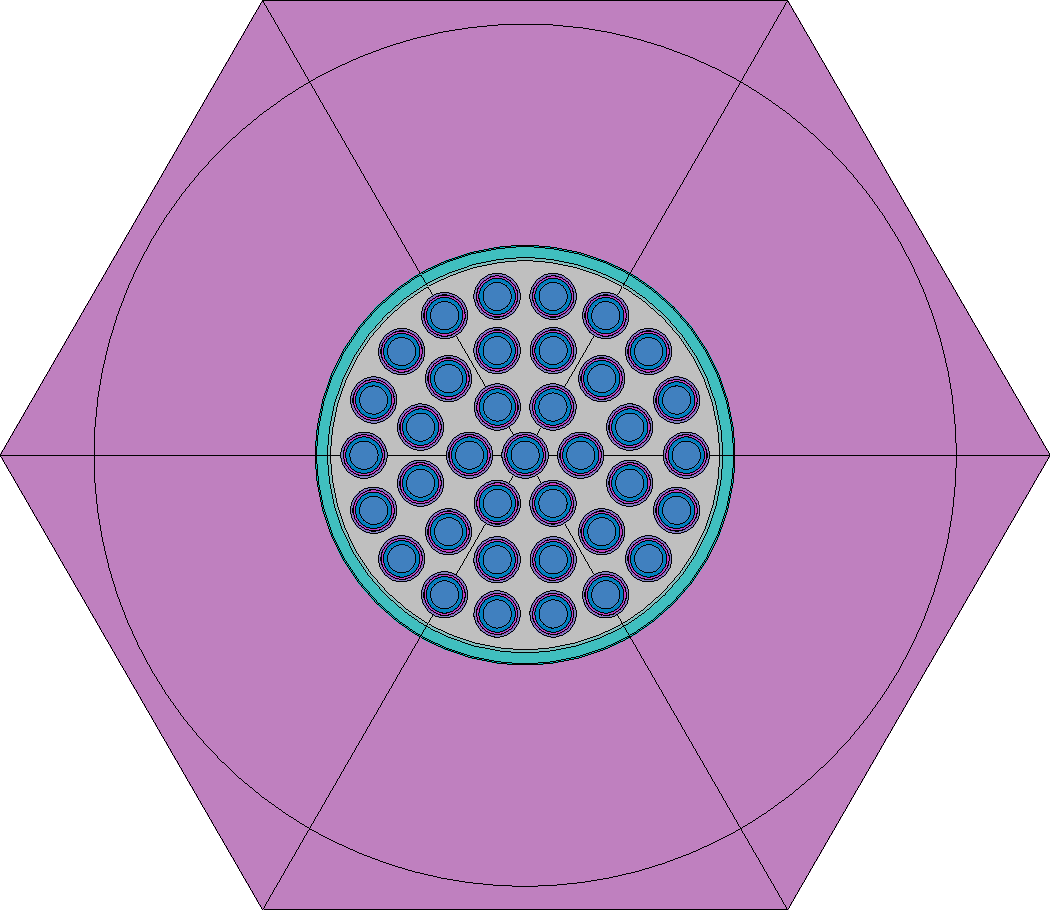
\includegraphics[width=0.35\linewidth]{imagenes/HexGeoMix_S-nxt.pdf}} 
  \subfloat[\label{fig:geo_t-nxt}]{ 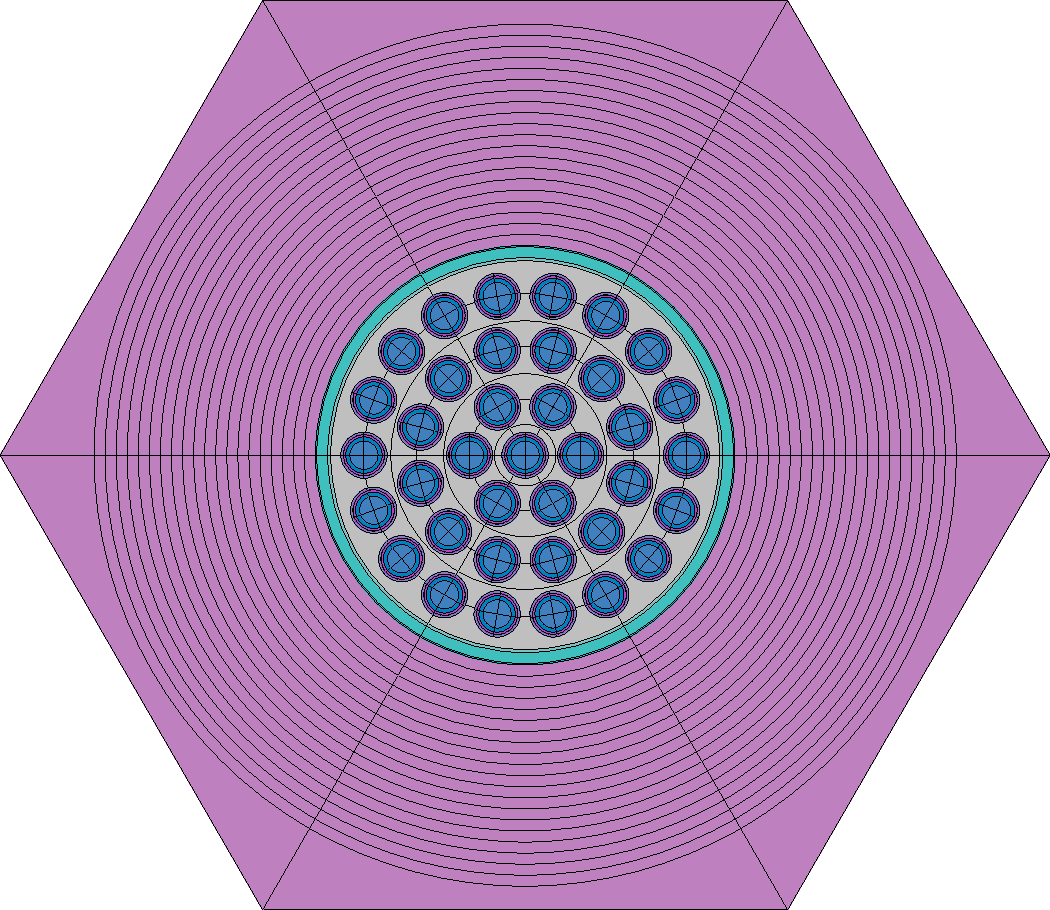
\includegraphics[width=0.35\linewidth]{imagenes/HexGeoMix_T-nxt.pdf}}\\
  \caption{Geometrías \texttt{HEXTCEL} para el cálculo de apantallamiento \texttt{geo_s} (\textbf{a}) y de transporte \texttt{geo_t} (\textbf{b}).}
  \label{fig:geos-nxt}
 \end{center}
\end{figure}

\begin{figure}[!h]
 \begin{center}
  \subfloat[\label{fig:geo_s-excelt}]{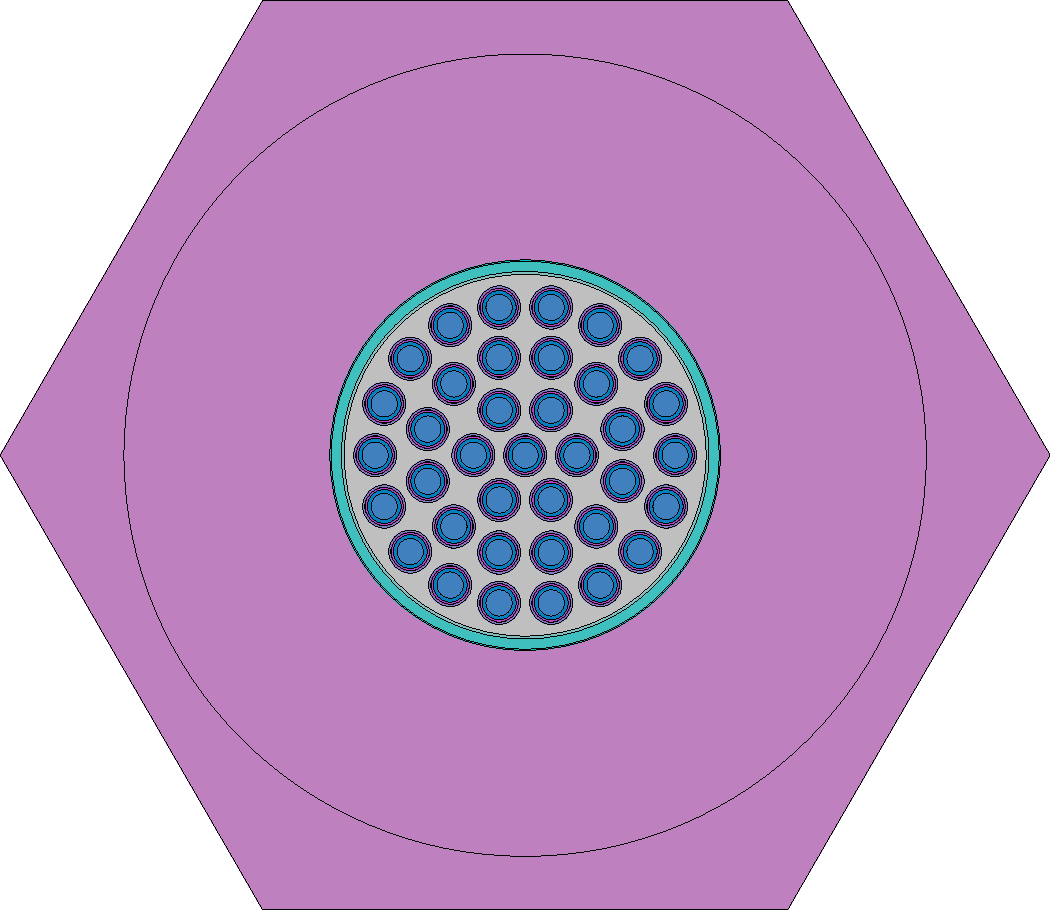
\includegraphics[width=0.35\linewidth]{imagenes/HexGeoMix_S-excelt.pdf}} 
  \subfloat[\label{fig:geo_t-excelt}]{ 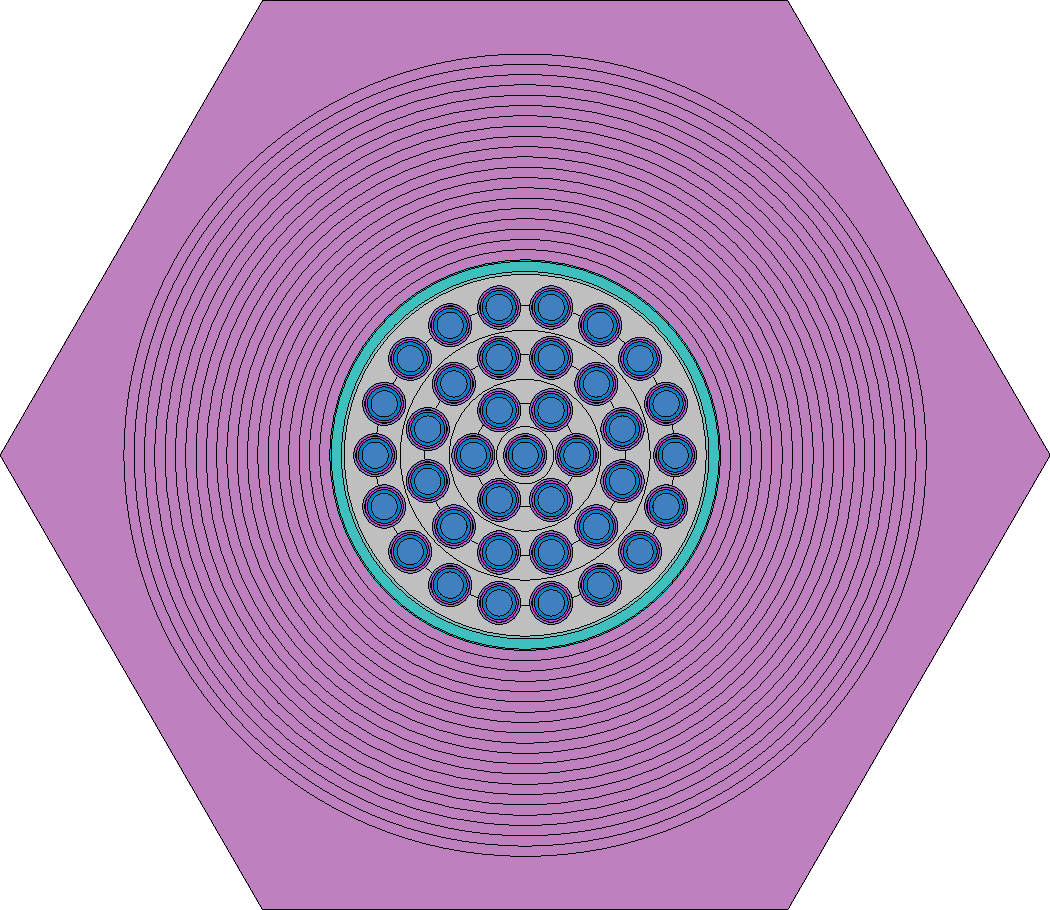
\includegraphics[width=0.35\linewidth]{imagenes/HexGeoMix_T-excelt.pdf}}\\
  \caption{Geometrías \texttt{HEXCEL} para el cálculo de apantallamiento \texttt{geo_s} (\textbf{a}) y de transporte \texttt{geo_t} (\textbf{b}).}
  \label{fig:geos-excelt}
 \end{center}
\end{figure}


\subsection{\emph{Tracking}}

Como ya se ha mencionado, son dos las geometrías que necesitan ser procesadas por un módulo de \emph{ray tracing} de DRAGON: una a utilizar en los cálculos de apantallamiento y otra en los de transporte. Si bien el \emph{ray tracing} debe realizarse una única vez, dependiendo de la cantidad de información generada por este, otros módulos verán su tiempo de calculo afectado considerablemente. Por ejemplo, la cantidad de probabilidades de colisión depende del número de regiones definidas o la cantidad de términos que contribuyen al cálculo de cada probabilidad de colisión depende de la densidad de rayos y de la cantidad de ángulos (ver Ref.~\cite{handbook-ingnuclear}). Por este motivo, es de suma importancia optimizar tanto las regiones como las densidades y los ángulos de las líneas del \emph{ray tracing}. La optimización de la densidad y los ángulos de las líneas resultó en \SI{5}{\per\centi\metre} y \SI{5}{\angle} respectivamente, tal como puede verse en la figura~\ref{fig:tracks}.

\begin{figure}[!h]
 \begin{center}
  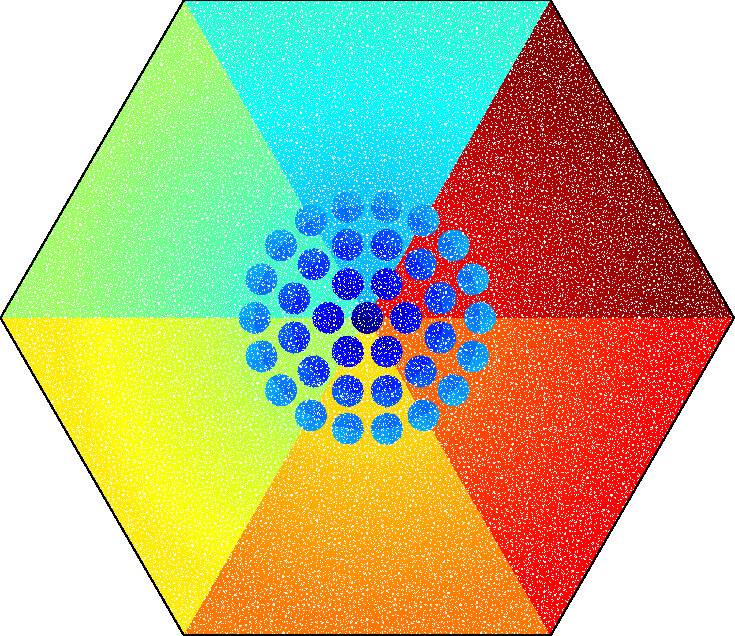
\includegraphics[width=0.4\linewidth]{imagenes/tracks.pdf}
 \end{center}
\caption{\label{fig:tracks} Líneas del \emph{ray tracing} empleado en las geometrías de apantallamiento y transporte.}
\end{figure}


\subsection{Quemado de referencia}

El quemado de referencia es un artilugio que permite realizar, en primera instancia, una evolución en quemado con ciertos parámetros globales $\vec{P_g}$ fijos. La información del depletado es almacenada en la estructura de datos \texttt{burnup} con el fin de poder realizar su posterior uso en un \emph{linear} (sec. \ref{subsec:linear-loop}) o \emph{nested loop} (\ref{subsec:nested-loop}). La lógica detrás de un quemado de referencia se presenta en el algoritmo~\ref{algo:reference-burnup}. 

\medskip
\begin{algorithm}[H]
 
 \Begin{
  comienzo del quemado de referencia: \emph{reference burnup loop}\;
  
  procedimiento \texttt{DefLib}: definir biblioteca\;
  procedimiento \texttt{CalcFlux}: apantallar y calcular transporte inicial (crear \texttt{flux} \emph{linked list})\;
  imprimir salida gráfica: \emph{fluxes}\;
  inicializar \texttt{burnup} \emph{linked list}\;
  condensar en energía y homogeneizar espacialmente\;
  
  \For{cada paso de quemado}{
   guardar información en \texttt{burnup} \emph{linked list} (tiempo inicial)\;
   depletar y posteriormente actualizar biblioteca al nuevo paso de quemado\;
   procedimiento \texttt{CalcFlux}: apantallar y calcular transporte (modificar \texttt{flux} \emph{linked list})\;
   condensar en energía y homogeneizar espacialmente\;
   guardar información en \texttt{burnup} \emph{linked list} (tiempo final)\;
  }
 }
 
 \caption{Quemado de referencia.\label{algo:reference-burnup}}
\end{algorithm}
\medskip


\subsection{Definición de biblioteca}

El procedimiento \texttt{DefLib.c2m} tiene como función definir tanto los materiales como sus propiedades. Se encuentra preparado para soportar bibliotecas con formato \texttt{DRAGLIB} (por ejemplo, \texttt{SHEM}) o \texttt{WIMSD4} (por ejemplo, \texttt{WLUP}). 

\medskip
\begin{algorithm}[H]
 
 \Begin{
  comienzo de la definición de la biblioteca\;
  
  leer parámetros de entrada para la biblioteca\;
  \uIf{la biblioteca es \texttt{WIMSD4}}{
   definir materiales con nomenclatura \texttt{WIMSD4} (saturados o a evolucionar según corresponda)\;
  }
  \uElseIf{la biblioteca es \texttt{DRAGLIB}}{
   definir materiales con nomenclatura \texttt{DRAGLIB} (saturados o a evolucionar según corresponda)\;
  }
  \Else{
  abortar\;
  }
  retornar \texttt{miclib} \emph{linked list}\;
 }
 
 \caption{Definición de biblioteca mediante procedimiento \texttt{DefLib}.\label{algo:deflib}}
\end{algorithm}
\medskip


\subsection{Cálculo de transporte}

El procedimiento \texttt{CalcFlux.c2m} permite resolver la ecuación de transporte mediante el método de las probabilidades de colisión obteniendo como resultado la distribución espacial y en energía del flujo escalar y el factor de multiplicación. El pseudocódigo detrás de ésta instrucción se detalla en el algoritmo~\ref{algo:calcflux}, mientras que la figura~\ref{fig:fluxes} representa la distribución espacial del flujo para un grupo rápido y otro térmico.

\medskip
\begin{algorithm}[H]
 
 \Begin{
  comienzo del cálculo de transporte\;
  
  leer parámetros de entrada para el cálculo\;
  \If{corresponde apantallar}{
   \eIf{es el primer paso de quemado}{
    apantallar y crear \texttt{miclib_s} \emph{linked list}\;
   }{
    apantallar y modificar \texttt{miclib_s} \emph{linked list}\;
   }
  }
  calcular probabilidades de colisión\;
  \eIf{es el primer paso de quemado}{
   calcular transporte y crear \texttt{flux} \emph{linked list}\;
  }{
   calcular transporte y modificar \texttt{flux} \emph{linked list}\;
  }
  extraer y retornar $k_{\infty}$\;
  retornar \texttt{miclib_s} y \texttt{flux} \emph{linked lists}\;
 }
 
 \caption{Cálculo de transporte mediante procedimiento \texttt{CalcFlux}.\label{algo:calcflux}}
\end{algorithm}
\medskip

\begin{figure}[!h]
 \begin{center}
  \subfloat[\label{fig:flux-1}]{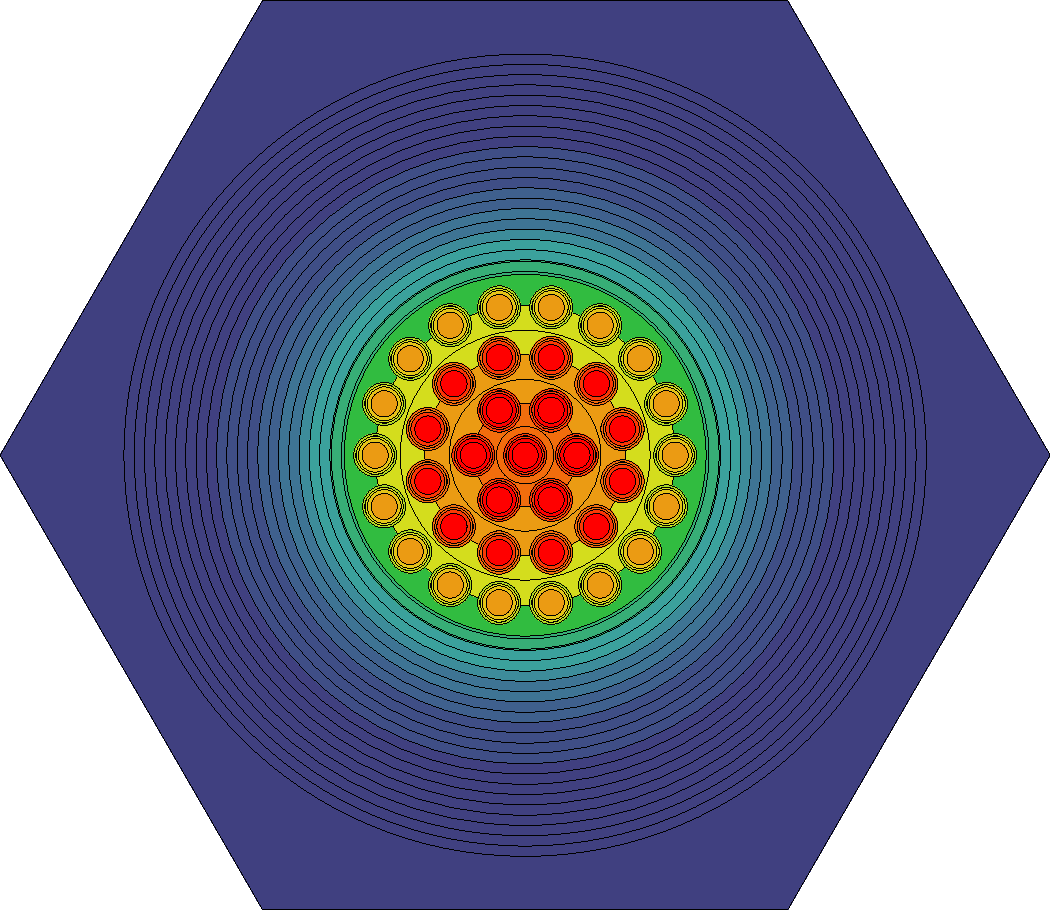
\includegraphics[width=0.4\linewidth]{imagenes/HexFlux_g1.pdf}}
  \newline
  \subfloat[\label{fig:flux-69}]{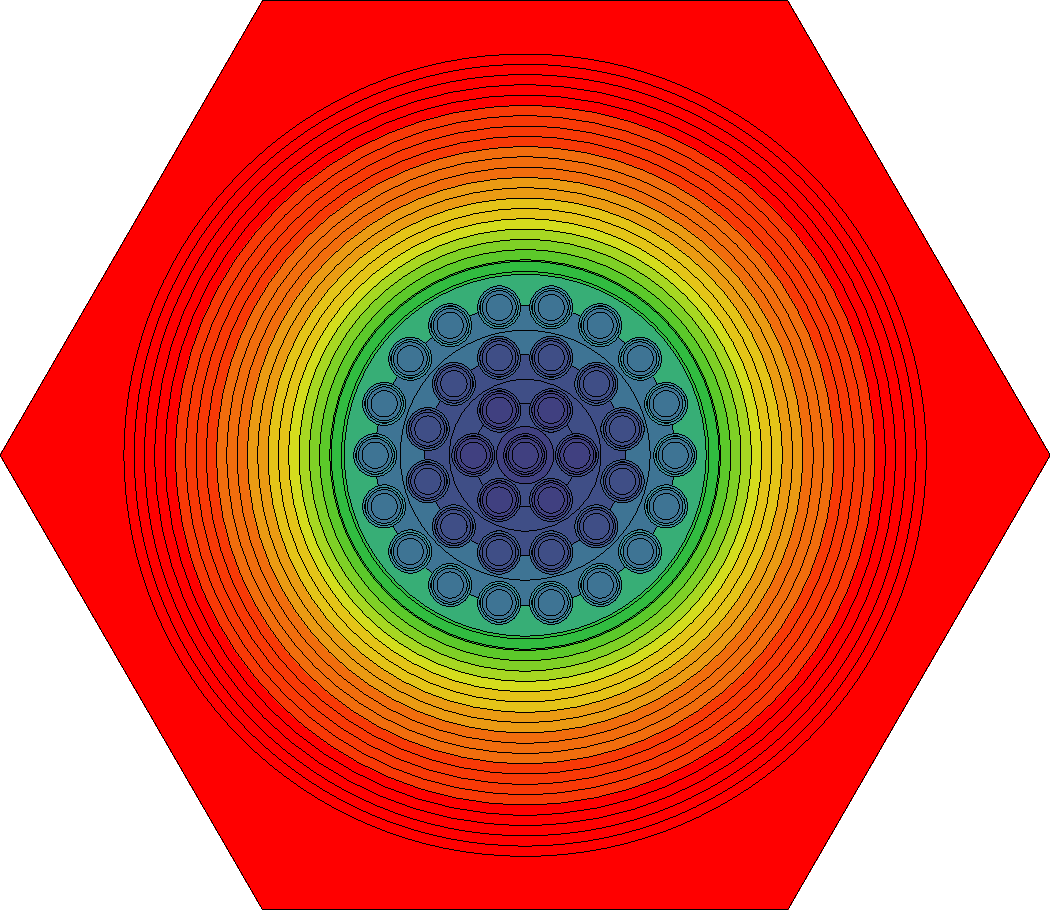
\includegraphics[width=0.4\linewidth]{imagenes/HexFlux_g69.pdf}}\\
  \caption{Distribución espacial del flujo pertenecientes al grupo más rápido (\textbf{a}) y más térmico (\textbf{b}) sin quemar.}
  \label{fig:fluxes}
 \end{center}
\end{figure}


\subsection{\emph{Linear loop}} \label{subsec:linear-loop}

Un \emph{linear loop} permite realizar las perturbaciones locales sobre algún parámetro de interés con el fin de obtener, para cada paso de quemado $Q_i$, la dependencia de las secciones eficaces con el parámetro en cuestión. Los algoritmos~\ref{algo:linear-pth} y~\ref{algo:linear-xenon} presentan la lógica detrás de una perturbación de este tipo para dos casos de interés: perturbación sobre un parámetro termohidráulico o sobre la concentración de xenón.

Como se detalla en los algoritmos~\ref{algo:linear-pth} y~\ref{algo:linear-xenon}, los resultados de un \emph{linear loop} se almacenan en un objeto \texttt{multicompo}. De esta manera, con un \emph{linear loop} se obtiene, para un mismo vector de parámetros globales $\vec{P^0_g}$, la dependencia de cada sección eficaz con el quemado y el parámetro local, es decir, $\Sigma_x \left( Q, P_l \right)$. Si bien la sección eficaz no varía linealmente con el quemado, puede ocurrir que si lo haga con el parámetro local. En este caso, para disminuir la dimensión de la interpolación del valor central de tabla $\Sigma_x \left( Q, \vec{P^0_g}, \vec{P^0_l} \right)$, se calcula y tabula la derivada $\partial\Sigma_x / \partial P_l$ en función del quemado.

\medskip
\begin{algorithm}[H]
 
 \Begin{
  comienzo de las perturbaciones lineales: \emph{linear loop}\;
  
  \For{cada perturbación local de parámetro termohidráulico}{
   procedimiento \texttt{DefLib}: definir biblioteca con parámetro perturbado\;
   
   \For{cada paso de quemado}{
    \eIf{es el primer paso de quemado}{
     procedimiento \texttt{CalcFlux}: apantallar y calcular transporte (crear \texttt{flux} \emph{linked list})\;
    }{
     actualizar concentraciones al paso de quemado correspondiente\;
     procedimiento \texttt{CalcFlux}: apantallar y calcular transporte (modificar \texttt{flux} \emph{linked list})\;
    }
    condensar en energía y homogeneizar espacialmente\;
    alimentar \texttt{multicompo} \emph{linked list}\;
   }
   eliminar \texttt{miclib}, \texttt{miclib_s} y \texttt{flux} \emph{linked lists}\;
  }
  
 }
 
 \caption{\emph{Linear loop} para perturbación de parámetro termohidráulico.\label{algo:linear-pth}}
\end{algorithm}
\medskip

\medskip
\begin{algorithm}[H]
 
 \Begin{
  comienzo de las perturbaciones lineales: \emph{linear loop}\;
  
  \For{cada perturbación local de la concentración de xenón}{
   procedimiento \texttt{DefLib}: definir biblioteca con parámetro perturbado\;
   
   \For{cada paso de quemado}{
    \eIf{es el primer paso de quemado}{
     procedimiento \texttt{CalcFlux}: apantallar y calcular transporte (crear \texttt{flux} \emph{linked list})\;
    }{
     actualizar concentraciones al paso de quemado correspondiente\;
     sobreescribir concentración de xenón al valor perturbado\;
     procedimiento \texttt{CalcFlux}: apantallar y calcular transporte (modificar \texttt{flux} \emph{linked list})\;
    }
    condensar en energía y homogeneizar espacialmente\;
    alimentar \texttt{multicompo} \emph{linked list}\;
   }
   eliminar \texttt{miclib}, \texttt{miclib_s} y \texttt{flux} \emph{linked lists}\;
  }
  
 }
 
 \caption{\emph{Linear loop} para perturbación de xenón.\label{algo:linear-xenon}}
\end{algorithm}
\medskip


\subsection{\emph{Nested loop}} \label{subsec:nested-loop}

Cuando la dependencia de la sección eficaz con ciertos parámetros locales no es ni separable ni lineal, es posible implementar un \emph{nested loop}. Esto permite, para un mismo vector de parámetros globales $\vec{P^0_g}$, definir exactamente a la sección eficaz, es decir, sin la necesidad aplicar alguna de las aproximaciones previamente descriptas en la ecuación~\ref{ec:aprox-general-1}. Por otra parte, con este tipo de \emph{loop} se obtienen las secciones eficaces para todas las combinaciones posibles dentro del rango de variación definido para cada parámetro, motivo por el cual es necesario utilizarlo únicamente en el caso que esto se requiera o implementar restricciones en el dominio (evitar el cálculo para ciertas combinaciones de parámetros que no posean sentido físico).

\medskip
\begin{algorithm}[H]
 
 \Begin{
  comienzo de las perturbaciones anidadas: \emph{nested loop}\;
  
  \For{cada perturbación local de parámetro termohidráulico $p_1$}{
   \For{cada perturbación local de parámetro termohidráulico $p_2$}{
    $\vdots$\\
    \For{cada perturbación local de parámetro termohidráulico $p_n$}{
     procedimiento \texttt{DefLib}: definir biblioteca con parámetros perturbados\;
     \For{cada paso de quemado}{
      \eIf{es el primer paso de quemado}{
       procedimiento \texttt{CalcFlux}: apantallar y calcular transporte (crear \texttt{flux} \emph{linked list})\;
      }{
       actualizar concentraciones al paso de quemado correspondiente\;
       procedimiento \texttt{CalcFlux}: apantallar y calcular transporte (modificar \texttt{flux} \emph{linked list})\;
      }
      condensar en energía y homogeneizar espacialmente\;
      alimentar \texttt{multicompo} \emph{linked list}\;
     }
     eliminar \texttt{miclib}, \texttt{miclib_s} y \texttt{flux} \emph{linked lists}\;
    }
   }
  }
 }
 
 \caption{\emph{Nested loop} para $n$ perturbaciones de parámetros termohidráulicos}
\end{algorithm}
\medskip

\section{Extracción de datos}

Los datos generados a partir de quemados de referencia, \emph{linear loops} o \emph{nested loops} son almacenados en estructuras de datos denominadas, usualmente, objetos \texttt{multicompo}. Estos objetos poseen un formato de datos que respeta cierta estructura que puede ser leída y procesada por las bibliotecas GanLib.

El Programa Cinético Espacial (PCE, Ref.~\cite{pumitacpl}) requiere de los siguientes datos para poder determinar tanto un estado estacionario de planta como la evolución de determinado transitorio:

\begin{itemize}
\renewcommand\labelitemi{$\cdot$}
 \item secciones eficaces condensadas y homogeneizadas, que incluyen coeficientes de difusión, absorciones, \emph{scattering} y fisiones rápidas y térmicas. En total son doce los valores a detallar: $D_{1}$, $D_{2}$, $\Sigma_{a1}$, $\Sigma_{12}$, $\Sigma_{21}$, $\Sigma_{a2}$, $\nu\Sigma_{f1}$, $\nu\Sigma_{f2}$, $e\Sigma_{f1}$, $e\Sigma_{f2}$, $\Sigma_{f1}$ y $\Sigma_{f2}$;
 \item constantes del xenón y iodo para la determinación de la dinámica de los mismos. Estas incluyen seis valores: \emph{yields} de fisión para el xenón y iodo (térmicos y rápidos) y las secciones eficaces microscópicas de absorción del xenón;
 \item derivadas de las secciones eficaces con respecto a los parámetros termohidráulicos y el xenón, que se determinan a partir del análisis de objetos \texttt{multicompo} con información acerca de las secciones eficaces detalladas en el primer ítem.
\end{itemize}

El algoritmo~\ref{algo:multicompo-extractor} detalla el pseudocódigo de las rutinas escritas en C para extraer la información almacenada en las estructuras de datos \texttt{multicompo} y generar archivos para definir funciones en formato wasora. Esto último es debido a que tanto la interpolación multidimensional de PCE o el análisis para calcular la dependencia lineal de las secciones eficaces con algún parámetro se realiza bajo esquemas que utilizan funciones de este tipo.

\medskip
\begin{algorithm}[H]
 
 \KwData{Archivo \texttt{ASCII} perteneciente a un objeto \texttt{multicompo} conteniendo las secciones eficaces pertinentes.}
 \KwResult{Archivo \texttt{ASCII} capaz de ser utilizado para definir funciones de secciones eficaces en wasora.}
 
 abrir archivo \texttt{ASCII} conteniendo el objeto \texttt{multicompo}\;
 definir archivo \texttt{ASCII} de salida\;
 verificar la consistencia con el número de cálculos esperados en el objeto \texttt{multicompo}\;
 leer puntos de definición de los cálculos\;
 \For{cada calculo contenido en el objeto \texttt{multicompo}}{
  imprimir puntos de definición\;
  \uIf{el objeto \texttt{multicompo} contiene información de la dinámica del iodo y xenón }{
   imprimir las seis constantes para la dinámica del iodo y xenón\;
  }
  \ElseIf{el objeto \texttt{multicompo} contiene información de secciones eficaces perturbadas}{
   imprimir las doce secciones eficaces\;
  }
 }
 
 \caption{Extracción de datos de objetos \texttt{multicompo}.\label{algo:multicompo-extractor}}
\end{algorithm}
\medskip

\section{Análisis de las dependencias globales y locales}
\label{sec:dependencias-globales-locales}

Con el objetivo de desarrollar en mayor profundidad la ecuación~\ref{ec:aprox-general-1} se presentan, a continuación, algunos conceptos que serán tenidos en cuenta a la hora de describir el esquema de la tabla de secciones eficaces detallada en la sección~\ref{sec:modelo-detallado}. Estos conceptos abarcan tanto la descripción de las diferentes aproximaciones así como también la repercusión de cada una de ellas en los cálculos a realizar en un código de celda.

En el caso más simple la dependencia de las secciones eficaces es solo función de un único parámetro $P$. La sección eficaz exacta para un dado estado corresponde a $\Sigma_x \left( Q, P_g, P_l \right)$. Obtener este valor en un código de celda requiere de un cálculo en el que se queme con $P_g$ y una vez en el paso de quemado correspondiente, se perturbe con $P_l$ (notar que si $P_l = P_g$, se corresponde a un caso sin perturbar). Si la dependencia con el parámetro local es lineal, podemos reducir la dimensión de la interpolación del valor central de tabla (se elimina la dependencia con $P_l$) de forma que 

\begin{equation} \label{ec:aprox-general-2}
% \begin{split}
 \Sigma_x \left( Q, P_g, P_l   \right) \approx 
 \Sigma_x \left( Q, P_g        \right)\bigg|_{P^0_l} +
 \frac{\partial\Sigma_x}{\partial P_l}\bigg|_{\left( Q, P_g, P^0_l \right)} \cdot \left(P_l - P^0_l \right).
% \end{split}
\end{equation}

\noindent
Teniendo en cuenta los temas abordados previamente, la estimación de la derivada $\partial\Sigma_x / \partial P_l \left( Q, P_g, P^0_l \right)$ se realiza a partir de un \emph{linear loop} sobre el parámetro en cuestión. A su vez, el nuevo valor central de tabla puede desdoblarse en dos términos, de manera que

\begin{equation} \label{ec:aprox-general-3}
% \begin{split}
 \Sigma_x \left( Q, P_g \right)\bigg|_{P^0_l} \approx
 \Sigma_x \left( Q \right)\bigg|_{\left( P^0_g, P^0_l \right)} +
 \frac{\partial\Sigma_x}{\partial P_g}\bigg|_{\left( Q, P^0_g, P^0_l \right)} \cdot \left(P_g - P^0_g \right).
% \end{split}
\end{equation}

\noindent
En este caso, una forma de estimar la derivada $\partial\Sigma_x / \partial P_g \left( Q, P^0_g, P^0_l \right)$ es a partir de numerosos cálculos con diferentes parámetros globales, quemados de referencia y \emph{linear loops}. Estos resultados permiten estimar tanto la derivada parcial en función del quemado con dirección al parámetro global como aquella con dirección al parámetro local. Las figuras~\ref{fig:global-local-pth-1}--\ref{fig:global-local-pth-3} resumen gráficamente estos conceptos descriptos. La figura~\ref{fig:global-local-pth-1} presenta una sección eficaz a quemado nulo. En este caso se evidencia que, debido a que no hay evolución en quemado, el valor de la sección eficaz no depende del parámetro global (es decir, no hubo evolución de los materiales) y solo depende de la condición local. La figura~\ref{fig:global-local-pth-2} demuestra que la dependencia con el parámetro global cobra importancia a mayores quemados debido a que la determinación de los materiales difiere según el parámetro global utilizado para evolucionar. Por último, la figura~\ref{fig:global-local-pth-3} tabula, a modo de resumen, las dependencias de la derivada en sentido del parámetro local y de la derivada direccional $\left( \partial\Sigma_x / \partial P_l + \partial\Sigma_x / \partial P_g \right)$ como funciones del quemado, pudiéndose ver fácilmente que a bajos quemados la derivada en el sentido del parámetro global es despreciable. De todas formas, a medida que el quemado incrementa, no es correcto desestimar la derivada en dirección del parámetro global. Este tema volverá a ser abordado más adelante en esta misma sección.

\begin{figure}[!h]
 \begin{center}
  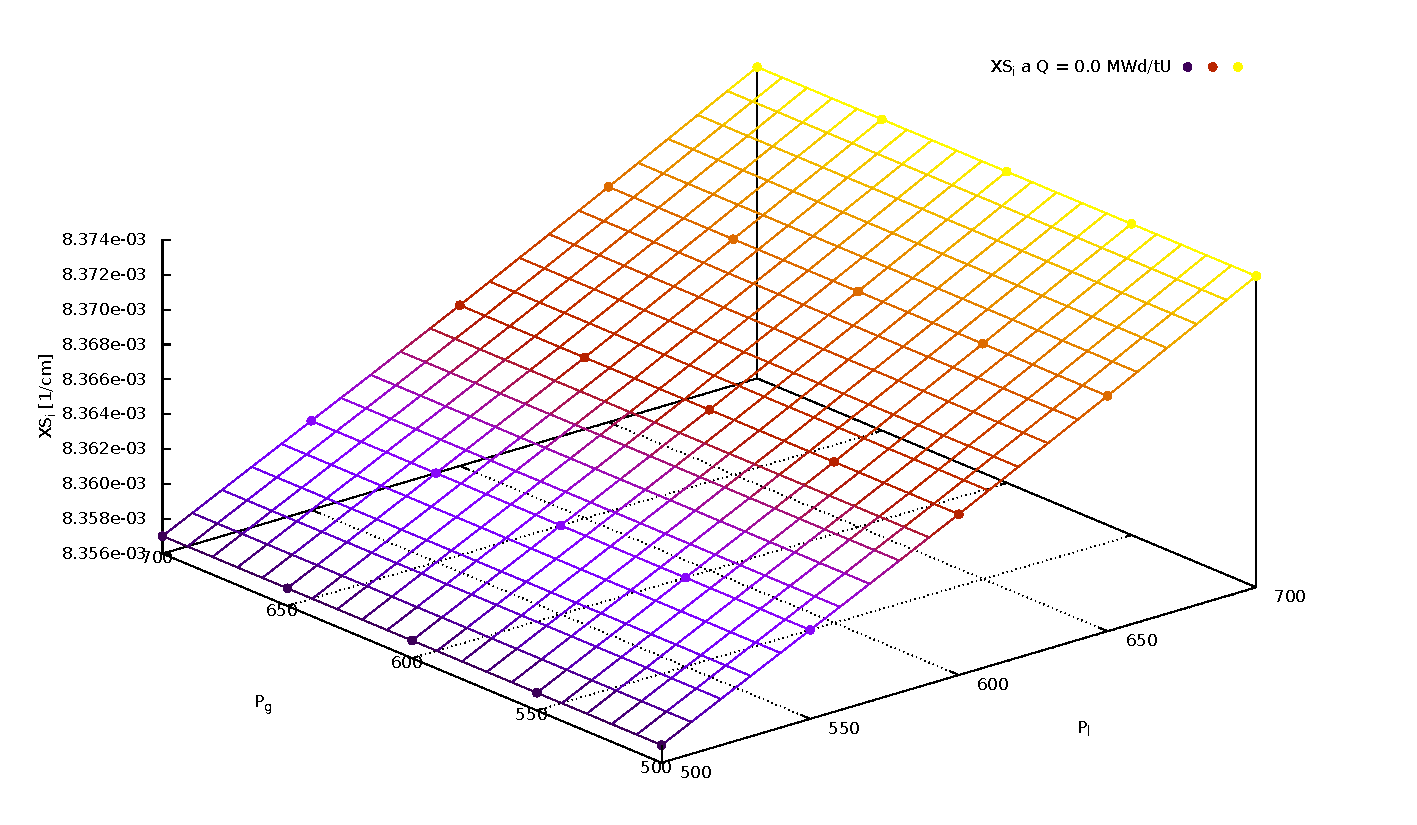
\includegraphics[width=1\linewidth]{graficos/dependencias-xs/XS1.pdf}
 \end{center}
\caption{\label{fig:global-local-pth-1} Esta figura presenta como es que la sección eficaz no varía en la dirección del parámetro global cuando se encuentra a $Q = \SI{0}{\mega\watt\day\per\tonne U}$.}
\end{figure}

\begin{figure}[!h]
 \begin{center}
  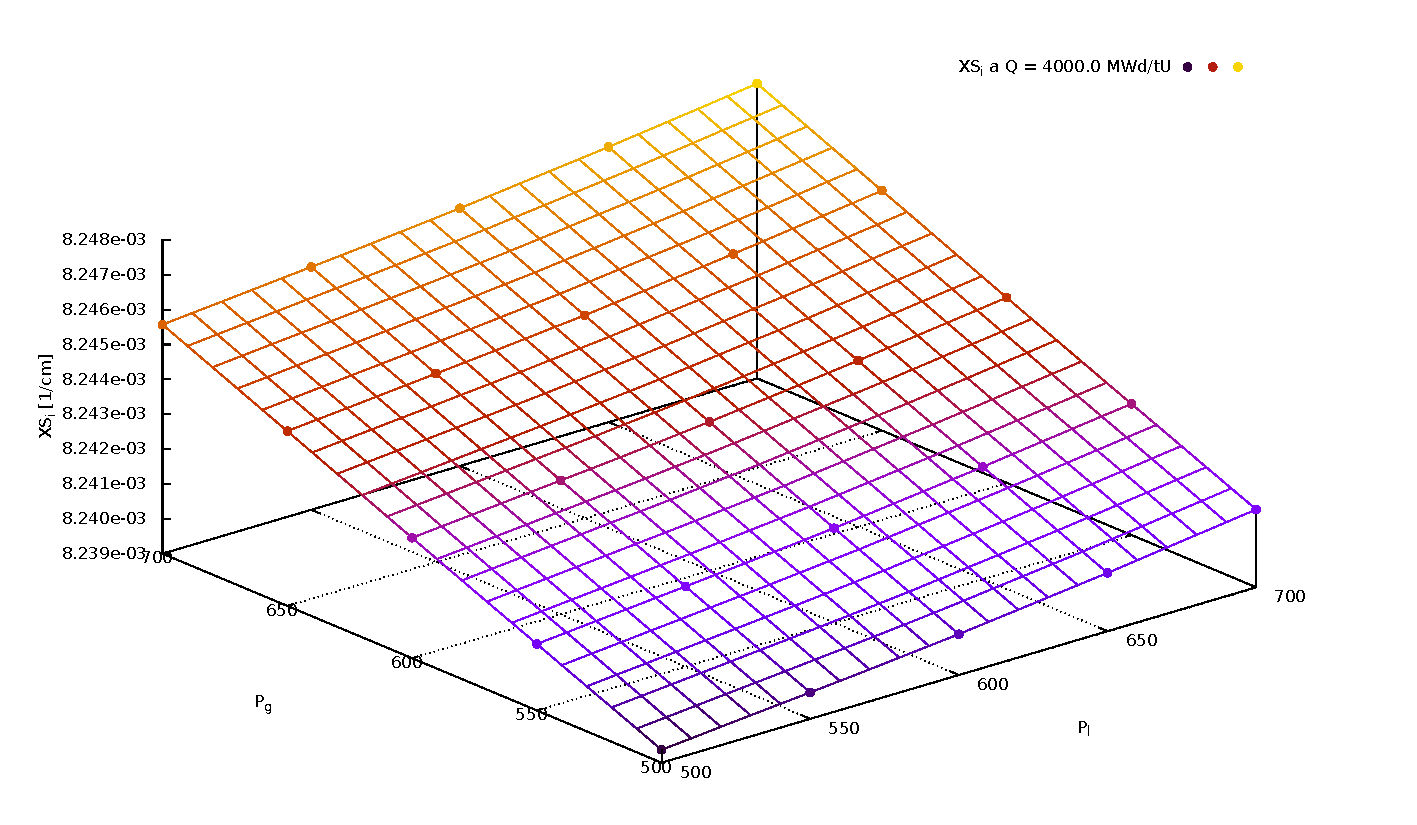
\includegraphics[width=1\linewidth]{graficos/dependencias-xs/XS2.pdf}
 \end{center}
\caption{\label{fig:global-local-pth-2} En este caso, a quemado $Q = \SI{4000}{\mega\watt\day\per\tonne U}$, la sección eficaz depende tanto del parámetro global como del local.}
\end{figure}

\begin{figure}[!h]
 \begin{center}
  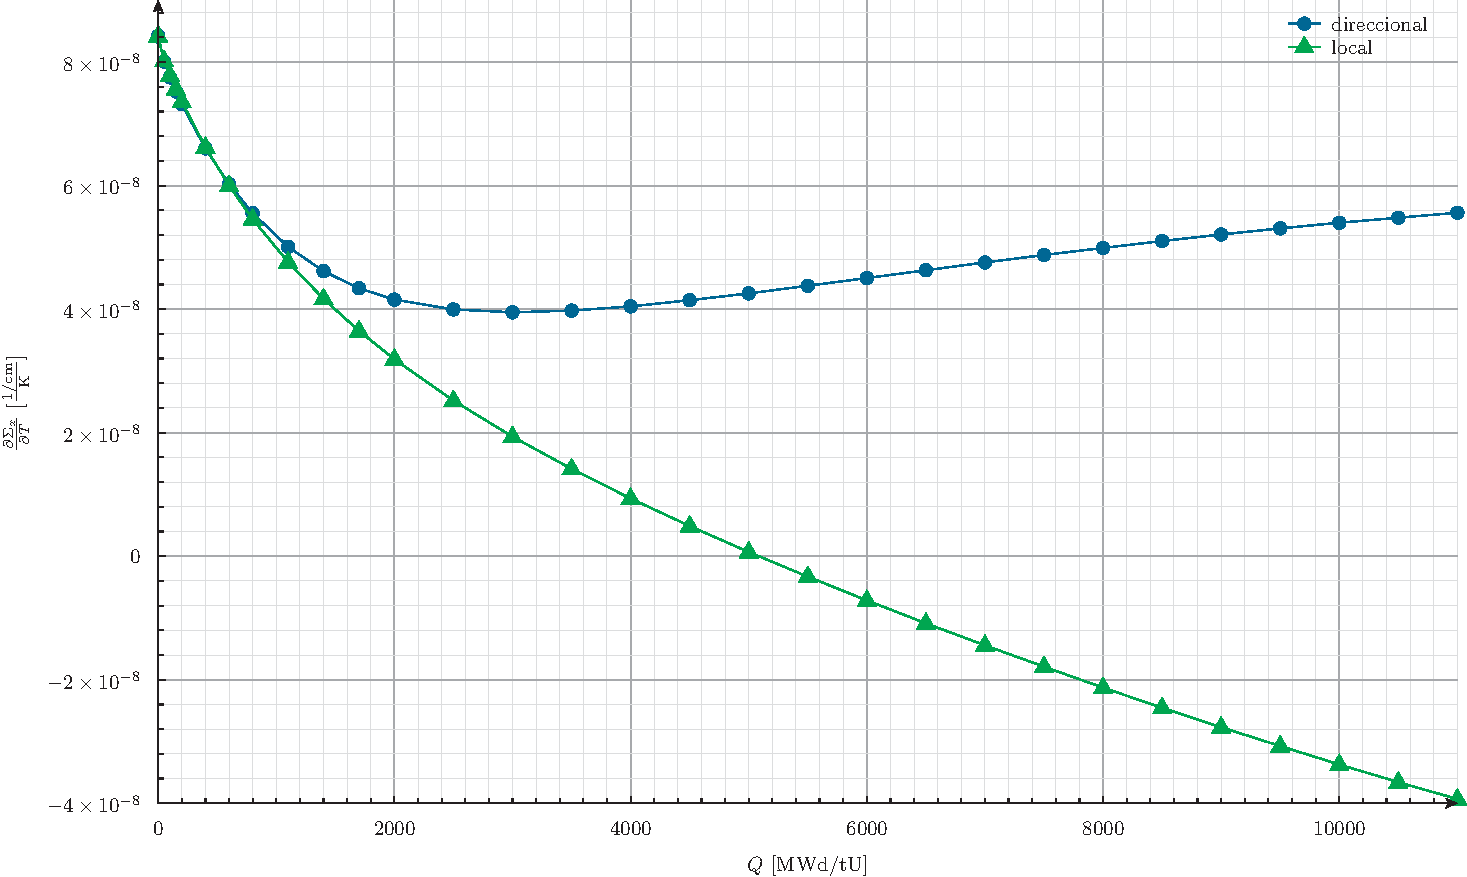
\includegraphics[width=0.9\linewidth]{graficos/dependencias-xs/dxs.pdf}
 \end{center}
\caption{\label{fig:global-local-pth-3} Derivada en la dirección del parámetro local y en la dirección de $P_g = P_l$ (direccional) de la sección eficaz en función del quemado. El hecho de que a bajos quemados ambas derivadas sean iguales refleja que la derivada en la dirección del parámetro global es despreciable. Posteriormente, esto deja de ser cierto, lo que indica que la derivada en el sentido del parámetro global no puede desestimarse.}
\end{figure}

Como ya se ha mencionado, en el caso que exista un parámetro con el que las secciones eficaces no varían linealmente, no es posible descomponer en un desarrollo de Taylor de primer orden al valor central de tabla. En este contexto, el valor central debe ser obtenido a partir de una interpolación que tenga en cuenta este parámetro. 

En el caso general, la tabla de secciones eficaces posee una dependencia con el quemado y los vectores $\vec{P_g}$ y $\vec{P_l}$. Traducir esto a un código de celda implica que, por cada combinación de parámetros globales, debe ejecutarse una corrida donde se realice un \emph{nested loop} sobre los parámetros locales y sus rangos de variación. Con el fin de disminuir la cantidad de cálculos de un \emph{nested loop} de gran dimensión, se aplica la aproximación desarrollada en la ecuación~\ref{ec:aprox-general-2} en aquellos parámetros que pueden ser considerados de forma aislada y cuya dependencia puede incorporarse con derivadas estimadas a partir de \emph{linear loops}. Sin embargo, aquellos parámetros con los que las secciones eficaces no presentan una dependencia lineal ni son separables deben incorporarse dentro del vector de interpolación, por lo que su dependencia es tabulada dentro del valor central. Por otro lado, con el fin de disminuir tanto la dimensión del vector de interpolación de la tabla como la cantidad de cálculos a realizar, la dependencia con los parámetros globales puede ser linealizada según la ecuación~\ref{ec:aprox-general-3}.

Es conveniente analizar dos situaciones de interés: la evaluación de las secciones eficaces durante la determinación de un estado estacionario de planta y durante un transitorio. En el caso estacionario se itera hasta encontrar las distribuciones de parámetros globales y locales, teniendo en cuenta que ambas son iguales, es decir, $\vec{P_g} (\vec{x}) = \vec{P_l} (\vec{x}) = \vec{P} (\vec{x})$. Si además se suponen perturbaciones separables y linealizables, la ecuación~\ref{ec:aprox-general-1} resulta en

\begin{equation} \label{ec:aprox-general-4}
% \begin{split}
 \Sigma^{\text{est}}_x \left( Q, \vec{P^{\text{est}}_g}, \vec{P^{\text{est}}_l} \right) \approx
 \Sigma_x \left( Q, \vec{P^0}, \vec{P^0} \right) + 
 \sum_{k = 1}^{N_P}{\left( \frac{\partial\Sigma_x}{\partial P_{g,k}} + \frac{\partial\Sigma_x}{\partial P_{l,k}} \right)\bigg|_{\left( Q, \vec{P^0}, \vec{P^0} \right)} \cdot \left(P^{\text{est}}_k - P^0_k \right) },
% \end{split}
\end{equation}

\noindent
donde la suma de ambas derivadas parciales da como resultado la derivada direccional en el sentido de $P_{g,k} = P_{l,k}$. 

Durante un transitorio, la sección eficaz se evalúa a partir del valor obtenido en el estacionario más las perturbaciones locales que correspondan (suponiendo que éstas son separables y linealizables), es decir:

\begin{equation} \label{ec:aprox-general-5}
% \begin{split}
 \Sigma^{\text{tr}}_x \left( Q, \vec{P^{\text{est}}_g}, \vec{P^{\text{tr}}_l} \right) \approx 
 \Sigma^{\text{est}}_x \left( Q, \vec{P^{\text{est}}_g}, \vec{P^{\text{est}}_l} \right) + 
 \sum_{k = 1}^{N_P}{\frac{\partial\Sigma_x}{\partial P_{l,k}}\bigg|_{\left( Q, \vec{P^0}, \vec{P^0} \right)} \cdot \left(P^{\text{tr}}_{l,k} - P^{\text{est}}_{l,k} \right) }.
% \end{split}
\end{equation}

\noindent
Analizando las ecuaciones~\ref{ec:aprox-general-4} y~\ref{ec:aprox-general-5}, si la derivada en la dirección del parámetro global es despreciable frente a la derivada en la dirección del parámetro local, la determinación de la sección eficaz tanto en un estacionario y como en un transitorio se realiza de la misma forma:

\begin{equation} \label{ec:aprox-general-6}
% \begin{split}
 \Sigma_x \left( Q, \vec{P_g}, \vec{P_l} \right) \approx 
 \Sigma_x \left( Q, \vec{P^0}, \vec{P^0} \right) + 
 \sum_{k = 1}^{N_P}{\frac{\partial\Sigma_x}{\partial P_{l,k}}\bigg|_{\left( Q, \vec{P^0}, \vec{P^0} \right)} \cdot \left(P_{l,k} - P^0_{l,k} \right) }.
% \end{split}
\end{equation}

\noindent
Sin embargo, esta última aproximación no ocurre para casi ninguno de los parámetros.


\section{Modelo detallado}
\label{sec:modelo-detallado}

En esta sección se describen, en primera instancia, las consideraciones físicas y matemáticas del esquema detallado de secciones eficaces de CNA2. Por otro lado, y sólo a título informativo, se detalla la forma de obtener la tabla de múltiples parámetros a utilizar en PCE haciendo uso de diferentes programas y \emph{scripts}. A su vez, con el fin de implementar los esquemas de generación de tablas de múltiples parámetros se incluye el desarrollo del pseudocódigo de cada uno de los \emph{scripts}.

% {\color{blue}poner graficos de resultados de XS frente a los de wims de antes!}

\subsection{Descripción}

La aplicación de la ecuación~\ref{ec:aprox-general-1} a un modelo de reactor requiere seleccionar adecuadamente los parámetros y sus rangos de variación. Por este motivo, es de suma importancia estudiar la dependencia de las secciones eficaces con cada uno de los parámetros de entrada. El caso con mayor grado de detalle consiste en una tabla de secciones eficaces con los siguientes parámetros de entrada: quemado, temperaturas y densidades globales y locales del refrigerante y moderador, perfil de temperatura global y local del combustible y concentración de xenón global y local. La cantidad de combinaciones posibles entre estos parámetros equivale al producto de la discretización de cada uno de ellos. Obtener esta información no sólo requiere de una gran cantidad de cálculos de celda, si no que también de una costosa implementación computacional en un código de núcleo. Con el fin de calcular una tabla de secciones eficaces con este grado de detalle, pero evitando la costosa implementación, se seleccionaron los parámetros de entrada presentes en la tabla~\ref{table:modelo-detallado} y detallados a continuación.

{
\begin{table}[h!]
\begin{center}
\begin{tabular}{|c|c|c|c|c|c|c|c|c|c|}
\hline
         & \multicolumn{4}{c|}{PL}                  & \multicolumn{2}{c|}{PG} & \multicolumn{3}{c|}{Funciones}\\
\hline
$Q$      & $\theta_{1}$ & $\theta_{2}$ & $\theta_{3}$ & $\theta_{4}$ & $q\prime$      & $z$      & $\Sigma_x$ & $C_{\text{Xe}}$ y $C_{\text{I}}$ & $\left( \partial\Sigma_x / \partial P \right)_{l,k}$\\
\hline
$\vdots$ & $\vdots$     & $\vdots$     & $\vdots$     & $\vdots$     & $\vdots$  & $\vdots$ & $\vdots$   & $\vdots$                         & $\vdots$\\
\hline
\end{tabular}
\caption{\label{table:modelo-detallado} Esquema conceptual de la tabla de secciones eficaces para el modelo detallado.}
\end{center}
\end{table}
}

\begin{itemize}
\renewcommand\labelitemi{$\cdot$}
 \item PL: parámetros locales;
 \item PG: parámetros globales;
 \item $Q$: quemado;
 \item $\theta_i$: temperatura media local y adimensional del volumen anular $i$ del combustible, tal que
 \begin{equation*}
  \theta_i = \frac{T_i - \SI{273.15}{\kelvin}}{T^{\text{est}}_i - \SI{273.15}{\kelvin}};
 \end{equation*}
 \item $q\prime$: potencia lineal global;
 \item $z$: representa la posición axial en el núcleo con el fin de determinar temperaturas y densidades globales y estacionarias del refrigerante y moderador{\footnote{El parámetro $z$ toma como valor un entero entre \num{1} y \num{10} que permite determinar las propiedades medias correspondientes a los trozos $\text{tr}_1 = \left( 2z-1 \right)$ y $\text{tr}_2 = 2z$ del reticulado de representación del reactor modelado en PCE.}}. Por este motivo, previamente deben conocerse las distribuciones estacionarias de temperaturas y densidades, lo que implica que el proceso para generar esta tabla es iterativo entre la determinación de un estado estacionario de núcleo y los cálculos de celda;
 \item $\Sigma_x$: valor central de tabla;
 \item $C_{\text{Xe}}$ y $C_{\text{I}}$: constantes para determinar la dinámica del xenón y iodo; y
 \item $\left( \partial\Sigma_x / \partial P \right)_{l,k}$: derivadas locales de las secciones eficaces respecto al parámetro $P_k$: xenón, temperatura o densidad del refrigerante y moderador.
\end{itemize}


En primer lugar se analizan los parámetros globales dejando a un lado los locales. Los parámetros globales son la potencia lineal $q\prime$ y una magnitud $z$ que representa la posición axial en el núcleo. Esta posición axial permite determinar el valor de las temperaturas y densidades globales del refrigerante y moderador si se conoce la distribución axial estacionaria de los mismos. A su vez, la temperatura del refrigerante junto a la potencia lineal y un modelo de combustible son utilizados para estimar el perfil de temperatura dentro de la pastilla (Ref.~\cite{modelos-pastilla-relap}). De esta forma, la elección de estos dos parámetros globales permite estimar a todos los parámetros globales reduciendo considerablemente los tiempos de cálculo debido a que cada combinación posible de parámetros globales $\vec{P_g}$ requiere de una ejecución del código de celda con el correspondiente quemado de referencia y, según corresponda, un \emph{nested} o \emph{linear loop} para las perturbaciones locales.

La determinación del estado estacionario se lleva a cabo únicamente a partir de los valores centrales de tabla (a excepción del xenón, que es incorporado de forma aislada) sin perturbar. Esto significa que es necesario utilizar únicamente el valor de $\Sigma_x \left( Q, \vec{P_g}, \vec{P_g} \right) = \Sigma_x \left( Q, q\prime, z, \theta_i = \num{1} \right)$, obtenido a partir de una interpolación lineal de $n = \num{7}$ parámetros que toma en cuenta todas las posibles combinaciones entre ellos. El xenón estacionario es incorporado mediante la derivada en la dirección del parámetro local, debido a que la derivada en la dirección del parámetro global es despreciable (ver ecuación~\ref{ec:aprox-general-4}), tal como puede verse en la figura~\ref{fig:dependencias-xenon}. La siguiente ecuación resume la forma de computar las secciones eficaces estacionarias:

\begin{equation} \label{ec:aprox-general-7}
% \begin{split}
 \Sigma^{\text{est}}_x \left( Q, \vec{P^{\text{est}}_g}, \vec{P^{\text{est}}_g} \right) \approx
 \Sigma_x \left( Q, q\prime_{\text{est}}, z_{\text{est}}, \theta^{\text{est}}_i = \num{1} \right) + 
 \frac{\partial\Sigma_x}{\partial \text{Xe}_l}\bigg|_{\left( Q, q\prime_{\text{est}}, z_{\text{est}} \right)} \cdot \left( \text{Xe}^{\text{est}} - \text{Xe}^0 \right).
% \end{split}
\end{equation}

\begin{figure}[!h]
 \begin{center}
  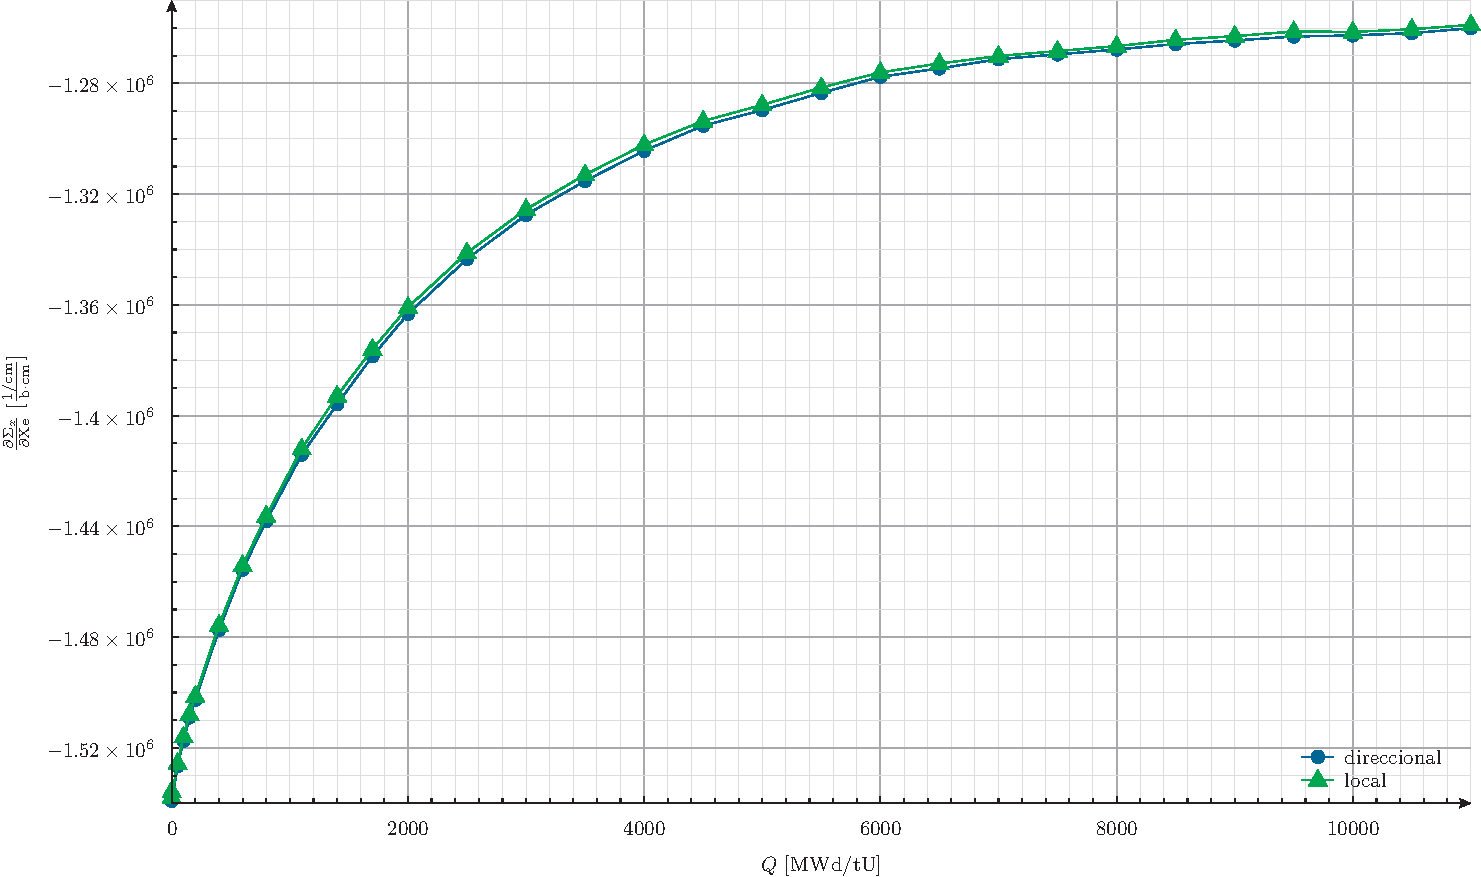
\includegraphics[width=0.75\linewidth]{graficos/dependencia-dxs-xenon/dxs.pdf}
 \end{center}
\caption{\label{fig:dependencias-xenon} Derivada en la dirección del xenón local y en la dirección de $\text{Xe}_g = \text{Xe}_l$ (direccional) de la sección eficaz en función del quemado. El hecho de que ambas derivadas sean prácticamente iguales refleja que la derivada en la dirección del xenón global es despreciable. Si bien estas curvas corresponden a la sección eficaz de absorciones térmicas, lo mismo ocurre para el resto de las secciones eficaces.}
\end{figure}

En un transitorio, los valores de $\theta_i$ no equivalen necesariamente a \num{1}. Por otro lado, las dependencias sobre el xenón y las temperaturas y densidades del refrigerante y moderador son tenidas en cuenta a partir de derivadas locales, tal como se muestra en el segundo término de la ecuación~\ref{ec:aprox-general-5}. Estas consideraciones resultan en la siguiente aproximación para la determinación de las secciones eficaces transitorias:

\begin{multline} \label{ec:aprox-general-8}
% \begin{split}
 \Sigma^{\text{tr}}_x \left( Q, \vec{P^{\text{est}}_g}, \vec{P^{\text{tr}}_l} \right) \approx
 \Sigma_x \left( Q, q\prime_{\text{est}}, z_{\text{est}}, \theta^{\text{tr}}_1, \theta^{\text{tr}}_2, \theta^{\text{tr}}_3, \theta^{\text{tr}}_4 \right) + \\
 \frac{\partial\Sigma_x}{\partial \text{Xe}_l}\bigg|_{\left( Q, q\prime_{\text{est}}, z_{\text{est}} \right)} \cdot \left( \text{Xe}^{\text{tr}}_l - \text{Xe}^0 \right) +
 \sum_{k = 1}^{N_{P}}{\frac{\partial\Sigma_x}{\partial P_{l,k}}\bigg|_{\left( Q, q\prime_{\text{est}}, z_{\text{est}} \right)} \cdot \left(P^{\text{tr}}_{l,k} - P^{\text{est}}_{l,k} \right)}.
% \end{split}
\end{multline}

\noindent
En la siguiente sección se detalla la forma en que se determinan el valor central de tabla, las constantes del xenón y iodo y las derivadas con respecto a los parámetros previamente mencionados a partir de entradas de DRAGON y códigos y \emph{scripts} que post procesan los resultados.


\subsection{Generación}

Conceptualmente, la generación de la tabla de secciones eficaces requiere de la utilización de todos los temas abordados previamente. Estas tareas se han automatizado dado que se requiere de la producción y análisis de una gran cantidad de datos. En esta sección se describe la forma de elaborar la tabla a emplear en el modelo detallado de la planta a partir de una serie de \emph{scripts} que ejecutan diferentes códigos e instrucciones.

La tabla~\ref{table:modelo-detallado} muestra qué valores se precisan obtener, por lo que se detallará la forma de calcular la información necesaria para determinar tanto los valores centrales de tabla $\Sigma_x$, las constantes del xenón y iodo ($C_{\text{Xe}}$ y $C_{\text{I}}$) y las derivadas locales de las secciones eficaces respecto al parámetro $P_k$ $\left( \partial\Sigma_x / \partial P \right)_{l,k}$ a partir de un único \emph{script} descripto en el algoritmo~\ref{algo:run-dragons}.

En primer lugar, la llamada al \emph{script} \texttt{run.sh} sin argumentos devolverá el \emph{usage} del mismo, esto es:

\begin{lstlisting}[style=bash_tecna]
$ ./run.sh 

  usage: ./run.sh <library_name> <tipo_de_calculo> [<parametro_th>] 
    donde library_name es el nombre de la librería a utilizar y ubicada dentro del directorio libraries,
    y tipo_de_calculo corresponde a nested-loop, xenon-dynamics, xenon-derivs o pth-derivs. 
    En el último caso, el parametro_th equivalente a trefr, drefr, tmod, o dmod debe ser especificado.
    Obs: las combinaciones sobre los parámetros globales son definidas en header.sh

\end{lstlisting}

Una vez especificada la biblioteca y definidas las combinaciones sobre los parámetros globales en el archivo \texttt{header.sh} es necesario especificar el tipo de cálculo. Para obtener los valores centrales de tabla, se ejecuta un tipo de cálculo \texttt{nested-loop}:

\begin{lstlisting}[style=bash_tecna]
$ ./run.sh IAEA-E6 nested-loop
\end{lstlisting}

\noindent
Estas ejecuciones serán paralelizadas y las salidas almacenadas en el directorio \texttt{outputs} bajo un nombre específico. Por otro lado, para obtener los datos necesarios para las $C_{\text{Xe}}$ y $C_{\text{I}}$ se realiza:

\begin{lstlisting}[style=bash_tecna]
$ ./run.sh IAEA-E6 xenon-dynamics
\end{lstlisting}

Por último, los datos necesarios para obtener posteriormente las derivadas (mediante el \emph{script} \texttt{multitable.sh} detallado en el algoritmo~\ref{algo:multitabla-detallada}) respecto al xenón o parámetros termohidráulicos se realiza, respectivamente:

\begin{lstlisting}[style=bash_tecna]
$ ./run.sh IAEA-E6 xenon-derivs
\end{lstlisting}

\begin{lstlisting}[style=bash_tecna]
$ ./run.sh IAEA-E6 pth-derivs trefr | drefr | tmod | dmod
\end{lstlisting}

Obtenidos todos los objetos \texttt{multicompo} almacenados en el directorio \texttt{outputs} bajo nombres específicos, se procede a realizar la tabla de secciones eficaces en el subdirectorio \texttt{multitable} mediante:

\begin{lstlisting}[style=bash_tecna]
$ ./multitable.sh
\end{lstlisting}

\begin{algorithm}[H]
 
 \KwData{Argumentos del \emph{script}.}
 \KwResult{Directorios conteniendo las salidas de DRAGON.}
 
 \If{no se proveyeron argumentos}{
   imprimir el \emph{usage} y abortar.
 }
 verificar argumentos provistos\;
 leer \texttt{header.sh} y definir combinaciones a realizar\;
 definir número de procesos a ejecutar en paralelo\;
 definir parámetros comunes a todos los procesos a ejecutar\;
 
 \For{cada altura de núcleo}{
  calcular parámetros termohidráulicos globales\;
  
  \For{cada potencia lineal}{
   calcular perfil de temperatura del combustible\;
   condensar perfil a volúmenes de DRAGON\;
   especificar nombre de directorio de corrida dependiendo del tipo de cálculo y parámetros globales\;
   
   \If{el tipo de cálculo requiere de perturbaciones locales}{
    definir perturbaciones locales dependiendo cual sea el parámetro\;
    reemplazar perturbaciones locales en el \emph{template} del \emph{input} que corresponda\;
   }
   
   reemplazar parámetros globales en el \emph{template} del procedimiento \texttt{DefParams}\;
   mover al directorio correspondiente el \emph{input} y los procedimientos\;
   ejecutar DRAGON\;
   
   \If{se alcanzó el número de procesos a paralelizar}{
    esperar la finalización de los procesos\;
   }
  }
 }
 
 \tcc{si el \# de cálculos no es múltiplo del \# de procesos a ejecutar en paralelo}
 \If{quedaron procesos lanzados}{
  esperar la finalización de los procesos\;
 }
 
 \caption{\emph{Script} \texttt{run.sh} para realizar las ejecuciones de DRAGON y así obtener los datos necesarios.\label{algo:run-dragons}}
\end{algorithm}

\medskip

\begin{algorithm}[H]
 
 \KwData{Objetos \texttt{multicompo}.}
 \KwResult{Tabla de secciones eficaces y sus derivadas.}
 
 leer \texttt{header.sh} y definir combinaciones a realizar\;
 verificar la existencia de todos los objetos \texttt{multicompo} necesarios\;
 
 \For{cada altura de núcleo}{
  \For{cada potencia lineal}{
   compilar rutinas de extracción de datos\;
   generar tabla parcial de valores centrales de tabla\;
   generar tabla parcial de constantes para la dinámica del iodo y xenón\;
   generar tabla parcial de derivadas respecto a la concentración de xenón\;
   generar tabla parcial de derivadas respecto a la temperatura de refrigerante\;
   generar tabla parcial de derivadas respecto a la densidad de refrigerante\;
   generar tabla parcial de derivadas respecto a la temperatura de moderador\;
   generar tabla parcial de derivadas respecto a la densidad de moderador\;
   unir tablas parciales para formar una `matriz fila' de la tabla final\;
   agregar `matriz fila' a la tabla final\;
   limpiar datos y archivos generados\;
  }
 }
 
 separar tabla final en secciones eficaces y sus derivadas\;
 \caption{\emph{Script} \texttt{multitable.sh} para obtener tabla de secciones eficaces.\label{algo:multitabla-detallada}}
\end{algorithm}


\label{lastpage}

% no bibliography by default to avoid problems with non-installed biber
\printbibliography

\end{document}

